% This must be in the first 5 lines to tell arXiv to use pdfLaTeX, which is strongly recommended.
\pdfoutput=1
% In particular, the hyperref package requires pdfLaTeX in order to break URLs across lines.

\documentclass[11pt]{article}

% Change "review" to "final" to generate the final (sometimes called camera-ready) version.
% Change to "preprint" to generate a non-anonymous version with page numbers.
\usepackage[final]{acl}

% Standard package includes
\usepackage{times}
\usepackage{latexsym}
\usepackage{xcolor}
\usepackage{xspace}
\usepackage{comment}
%\usepackage[colorlinks=true,urlcolor=black]{hyperref}
%\usepackage{subcaption,ragged2e}
\usepackage[normalem]{ulem}
\usepackage[utf8]{inputenc} % allow utf-8 input
\usepackage[T1]{fontenc}    % use 8-bit T1 fonts
\usepackage{url}
\usepackage{tikz}
\usepackage{enumitem}
\usetikzlibrary{positioning}
\usepackage{array}
\usepackage{booktabs}
% \usepackage{graphicx, subcaption,ragged2e}
\usepackage{wrapfig}
\usepackage{caption} % For a better control over table captions
\usepackage{floatrow}
\usepackage{listings}
\usepackage{adjustbox}
\usepackage{footnote}
\usepackage{multirow}
\usepackage{amsmath}
\usepackage{breakcites}
\usepackage{blindtext}
\usepackage{svg}
\usepackage[most]{tcolorbox}
\usepackage{fnbreak}
%\usepackage[square,numbers]{natbib}
%\setcitestyle{maxbibnames=3}

% For proper rendering and hyphenation of words containing Latin characters (including in bib files)
\usepackage[T1]{fontenc}
% For Vietnamese characters
% \usepackage[T5]{fontenc}
% See https://www.latex-project.org/help/documentation/encguide.pdf for other character sets

% This assumes your files are encoded as UTF8
\usepackage[utf8]{inputenc}

% This is not strictly necessary, and may be commented out,
% but it will improve the layout of the manuscript,
% and will typically save some space.
\usepackage{microtype}

% This is also not strictly necessary, and may be commented out.
% However, it will improve the aesthetics of text in
% the typewriter font.
\usepackage{inconsolata}

%Including images in your LaTeX document requires adding
%additional package(s)
\usepackage{graphicx}

% If the title and author information does not fit in the area allocated, uncomment the following
%
%\setlength\titlebox{<dim>}
%
% and set <dim> to something 5cm or larger.

% Below packages and commands inserted by Steven
\usepackage{tabularx} %note: inserted by Steven for table wrapping and other more advanced table commands
\usepackage{booktabs} %note: inserted by Steven for lines in tables, e.g. midrule
\usepackage{comment} %note: inserted by Steven for block commenting
\usepackage{wrapfig} %note: inserted by Steven for wrapping text around figures
%\usepackage{emerald}
%\usepackage[T1]{fontenc}
%\usepackage{lmodern}% http://ctan.org/pkg/lm
\newcommand{\latinword}[1]{\textsf{\itshape #1}}%
\usepackage{calligra}
\newcommand*\zapchan{\fontfamily{pzc}\selectfont}
\usepackage{aurical}

%note: below lines inserted by Steven for \n escapes
\newcommand*{\escape}[1]{\texttt{\textbackslash#1}}
\newcommand*{\escapeI}[1]{\texttt{\expandafter\string\csname #1\endcsname}}
\newcommand*{\escapeII}[1]{\texttt{\char`\\#1}}

\newcommand\blfootnote[1]{%
  \begingroup
  \renewcommand\thefootnote{}\footnote{#1}%
  \addtocounter{footnote}{-1}%
  \endgroup
}
\renewcommand{\UrlFont}{\ttfamily\small}
%\hypersetup{colorlinks,urlcolor={blue}}

\newenvironment{tight_enumerate}{
\begin{enumerate}[leftmargin=*]
  \setlength{\itemsep}{0pt}
  \setlength{\parskip}{0pt}
}{\end{enumerate}}
\newenvironment{tight_itemize}{
\begin{itemize}
  \setlength{\itemsep}{0pt}
  \setlength{\parskip}{0pt}
}{\end{itemize}}

\newenvironment{tightcenter}{%
  \setlength\topsep{0pt}
  \setlength\parskip{0pt}
  \begin{center}
}{%
  \end{center}
}

\makeatletter
\def\thickhline{%
  \noalign{\ifnum0=`}\fi\hrule \@height \thickarrayrulewidth \futurelet
   \reserved@a\@xthickhline}
\def\@xthickhline{\ifx\reserved@a\thickhline
               \vskip\doublerulesep
               \vskip-\thickarrayrulewidth
             \fi
      \ifnum0=`{\fi}}
\makeatother

\makeatletter
\newcommand\footnoteref[1]{\protected@xdef\@thefnmark{\ref{#1}}\@footnotemark}
\makeatother

\newlength{\thickarrayrulewidth}
\setlength{\thickarrayrulewidth}{2\arrayrulewidth}

\newcommand{\map}{\marginpar{MP}}

\newcommand*{\affmark}[1][*]{\textsuperscript{#1}}
% End of inserted packages and commands by Steven

%for color-coded comments:
\newcommand{\mostofa}[1]{{\color{blue}\bf [MP: #1]}\xspace}
\newcommand{\todo}[1]{{\color{red}\bf [TODO: #1]}\xspace}
\newcommand{\citereq}[1]{{\color{blue}\bf [CITE]}\xspace}
\newcommand{\shrimai}[1]{{\color{purple}\bf\small [Shrimai: #1]}\xspace}
\newcommand{\steven}[1]{\textcolor{magenta}{\bf\small [Steven: #1]}\xspace}
\newcommand{\kk}[1]{\textcolor{cyan}{\bf\small [Kezhi: #1]}\xspace}


\newcommand{\ccderiv}{$\mathtt{CC_{dv}}$\xspace}
\newcommand{\ccmq}{$\mathtt{CC}$-$\mathtt{Medium}$\xspace}
\newcommand{\ccmhq}{$\mathtt{CC}$-$\mathtt{Medium}$-$\mathtt{High}$\xspace}
\newcommand{\cchq}{$\mathtt{CC}$-$\mathtt{High}$\xspace}
\newcommand{\phaseone}{$\mathcal{P}_1$\xspace}
\newcommand{\phasetwo}{$\mathcal{P}_2$\xspace}

\newcommand{\gainRO}{$3.4$\%\xspace}
\newcommand{\gainND}{$17$\%\xspace}
\newcommand{\gainROND}{$13.2$\%\xspace}

\newcommand{\poneboneptwobone}{\phaseone-$\mathtt{Blend1}$-\phasetwo-$\mathtt{Blend1}$\xspace}
\newcommand{\poneboneptwobtwo}{\phaseone-$\mathtt{Blend1}$-\phasetwo-$\mathtt{Blend2}$\xspace}
\newcommand{\poneboneptwobthree}{\phaseone-$\mathtt{Blend1}$-\phasetwo-$\mathtt{Blend3}$\xspace}
\newcommand{\poneboneptwobfour}{\phaseone-$\mathtt{Blend1}$-\phasetwo-$\mathtt{Blend4}$\xspace}
\newcommand{\poneboneptwofive}{\phaseone-$\mathtt{Blend1}$-\phasetwo-$\mathtt{Blend5}$\xspace}

\newcommand{\ponebfourptwobone}{\phaseone-$\mathtt{Blend4}$-\phasetwo-$\mathtt{Blend1}$\xspace}
\newcommand{\ponebfourptwobtwo}{\phaseone-$\mathtt{Blend4}$-\phasetwo-$\mathtt{Blend2}$\xspace}
\newcommand{\ponebfourptwobthree}{\phaseone-$\mathtt{Blend4}$-\phasetwo-$\mathtt{Blend3}$\xspace}
\newcommand{\ponebfourptwobfour}{\phaseone-$\mathtt{Blend4}$-\phasetwo-$\mathtt{Blend4}$\xspace}
\newcommand{\ponebfourptwobfive}{\phaseone-$\mathtt{Blend4}$-\phasetwo-$\mathtt{Blend5}$\xspace}

\newcommand{\ptwobone}{\phasetwo-$\mathtt{Blend1}$\xspace}
\newcommand{\ptwobsix}{\phasetwo-$\mathtt{Blend6}$\xspace}
\newcommand{\ponebfourptwobsix}{\phaseone-$\mathtt{Blend4}$-\phasetwo-$\mathtt{Blend6}$\xspace}



%\title{Harnessing Data as Fuel: Boosting LLM Performance with Two-Phase Training}
\title{Maximize Your Data's Potential: Enhancing LLM \\Accuracy with Two-Phase Pretraining %\todo{Options for first part of the title: "Maximize Your Data's Potential", "Data-Driven Success", "Data as Fuel", "Maximizing Data as Fuel", "Leveraging Data as Fuel", "Harnessing Data as Fuel", "Optimizing Data as Fuel", "Smarter Data, Better Models", "The Art of Data", "From Data to Dominance", "Maximizing Data Potential", "Optimizing Data Use", "Train Smart, Not Hard"} \\ \steven{adjusted first part to focus more on "data" which is the main focus of our paper}
%\mostofa{remove '. Also word performance}
} 

%\steven{is "accuracy" really a good term here? maybe "capabilities" would be better if we want to avoid "performance"? accuracy seems too specific/particular, e.g. for certain tasks or capabilities, accuracy wouldn't be the metric used. i also feel it would be misunderstood by the general community compared to something like "performance" which is commonplace and refers to the LLM's overall capabilities. i know bryan doesn't like that word, but if we're publishing this publicly, i feel we need to take into account the general community's standards/vocabulary?}

%\title{Data Mixing \& Pretraining Strategies for Large Language Models \todo{placeholder title. possible candidates sent on slack}}

% Author information can be set in various styles:
% For several authors from the same institution:
% \author{Author 1 \and ... \and Author n \\
%         Address line \\ ... \\ Address line}
% if the names do not fit well on one line use
%         Author 1 \\ {\bf Author 2} \\ ... \\ {\bf Author n} \\
% For authors from different institutions:
% \author{Author 1 \\ Address line \\  ... \\ Address line
%         \And  ... \And
%         Author n \\ Address line \\ ... \\ Address line}
% To start a separate ``row'' of authors use \AND, as in
% \author{Author 1 \\ Address line \\  ... \\ Address line
%         \AND
%         Author 2 \\ Address line \\ ... \\ Address line \And
%         Author 3 \\ Address line \\ ... \\ Address line}

\author{Steven Y. Feng\thanks{equal contribution}$^{2}$\thanks{Work done during internship at NVIDIA}, Shrimai Prabhumoye$^{*}$$^{1,3}$, Kezhi Kong$^{1}$, Dan Su$^{1}$, \\ \textbf{Mostofa Patwary$^{1}$, Mohammad Shoeybi$^{1}$, Bryan Catanzaro$^{1}$} \\
NVIDIA$^{1}$, Stanford University$^{2}$, Boston University$^{3}$ \\
  \texttt{sprabhumoye@nvidia.com} \\}

%\author{
%  \textbf{First Author\textsuperscript{1}},
%  \textbf{Second Author\textsuperscript{1,2}},
%  \textbf{Third T. Author\textsuperscript{1}},
%  \textbf{Fourth Author\textsuperscript{1}},
%\\
%  \textbf{Fifth Author\textsuperscript{1,2}},
%  \textbf{Sixth Author\textsuperscript{1}},
%  \textbf{Seventh Author\textsuperscript{1}},
%  \textbf{Eighth Author \textsuperscript{1,2,3,4}},
%\\
%  \textbf{Ninth Author\textsuperscript{1}},
%  \textbf{Tenth Author\textsuperscript{1}},
%  \textbf{Eleventh E. Author\textsuperscript{1,2,3,4,5}},
%  \textbf{Twelfth Author\textsuperscript{1}},
%\\
%  \textbf{Thirteenth Author\textsuperscript{3}},
%  \textbf{Fourteenth F. Author\textsuperscript{2,4}},
%  \textbf{Fifteenth Author\textsuperscript{1}},
%  \textbf{Sixteenth Author\textsuperscript{1}},
%\\
%  \textbf{Seventeenth S. Author\textsuperscript{4,5}},
%  \textbf{Eighteenth Author\textsuperscript{3,4}},
%  \textbf{Nineteenth N. Author\textsuperscript{2,5}},
%  \textbf{Twentieth Author\textsuperscript{1}}
%\\
%\\
%  \textsuperscript{1}Affiliation 1,
%  \textsuperscript{2}Affiliation 2,
%  \textsuperscript{3}Affiliation 3,
%  \textsuperscript{4}Affiliation 4,
%  \textsuperscript{5}Affiliation 5
%\\
%  \small{
%    \textbf{Correspondence:} \href{mailto:email@domain}{email@domain}
%  }
%}

\begin{document}
\maketitle
\begin{abstract}
    Pretraining large language models effectively requires strategic data selection, blending and ordering. 
    %However, key model developers often do not disclose details about data mixes and ordering, and their generalizability to longer token horizons and larger model scales.
    However, key details about data mixtures especially their scalability to longer token horizons and larger model sizes remain underexplored due to limited disclosure by model developers.
    To address this, we formalize the concept of \textit{two-phase pretraining} and conduct an extensive systematic study on how to select and mix data to maximize model accuracies for the two phases.
    Our findings illustrate that a two-phase approach for pretraining outperforms random data ordering and natural distribution of tokens by \gainRO and \gainND on average accuracies.
    %a random data ordering by an average of \gainRO and a blend based on natural distribution of tokens (blend is not based on quality or epochs) by \gainND across downstream tasks.
    We provide in-depth guidance on crafting optimal blends based on quality of the data source and the number of epochs to be seen.
    We propose to design blends using downsampled data at a smaller scale of 1T tokens and then demonstrate effective scaling of our approach to larger token horizon of 15T tokens and larger model size of 25B model size.
    %\mostofa{mention larger tokens and larger token horizon and then add 15T and 25B as example}.
    %We provide in-depth guidance on crafting optimal blends for both the phases of pretraining, and determining the duration for each phase.
    %Additionally, we provide a comprehensive study on creating blends based on the quality of the data source including analysis of web crawl quality based data mixing.
    %We demonstrate how blends can be designed at a smaller scale of 1T tokens and then scaled to 15T tokens and 25B model size.
    %We demonstrate how these blends scale effectively to larger models and token budgets.  
    %Our findings show that a two-phase training approach starting with a more general data distribution followed by heavier amounts of math, code, and task data for the last 40\% of training maximizes performance across benchmarks and generalizes effectively to larger scales. 
    %Specifically, we find that starting with a more general data distribution followed by heavier amounts of math, code, and task data for the last 40\% of pretraining yields superior performance across benchmarks and generalizes effectively to larger scales. 
    These insights provide a series of steps practitioners can follow to design and scale their data blends.
   
\end{abstract}

%\shrimai{Add a range of how much improvement across blends}
%\shrimai{Connect contributions to abstract}

% \section{PLAN \& Notes}

% \begin{itemize}
%     \item in-depth analysis of data, findings, existing work shows upsampling is better at baseline
%     \item how much upsampling phase
%     \item quality of datasets: compare with medium and high quality crawl to determine quality. score-bucketing for crawl, Kezhi's graphs that show impact of different buckets, Dan's number of epochs expt, Dan's "within" crawl blend expts
%     \item Task oriented data: sft data, flan, gsm8k synthetic
%     \item epoch based analysis: how we decide how much to do high quality data is not dependent on percentage but dependent on epochs of high quality
%     \item scaled to 1.7T. answering the question: how do blends scale over token horizon
%     \item Potentially: scaled to 25B model: how do blends scale to different model sizes
%     \item Potentially: how eval tasks evolve over time
% \end{itemize}

% Expts to do

% \begin{enumerate}
%     \item 25B scaling expt [Shrimai]
%     \item One randomized expt [Shrimai]
%     \item remaining SFT expts (e.g. phase 3) [Kezhi]
%     \item MAYBE: epoch 1, 2, 4 for math and code in phase 2 [Shrimai]
%     \item MAYBE: upsampling at beginning (phase 2 --> phase 1) [??]
%     \item MAYBE: missing numbers for eval tasks over time [Shrimai]
% \end{enumerate}

% Contributions
% \begin{itemize}
%     \item 2 phased approach. Maybe 3 phase SFT part    
% \end{itemize}

% \begin{itemize}
%     \item Lot of work on llms but no understanding of the blends
%     \item Finewebedu gives insight into quality of crawl but not how to use it effectively. We show study on indepth understanding of crawl, how many epochs of crawl to use and how to blend.
%     \item We compare all datasets with crawl to judge their quality. Kezhi's work on books
% \end{itemize}


\section{Introduction}
%TODO: Steven

\begin{comment}
\subsection{Motivation}
\begin{itemize}
    \item Existing works like Llama 3.1 highlight the effectiveness of upsampling, but not details of the exact blends and experiments. What exactly works and why/how?
    \item Despite model and token scaling, we lack downstream accuracy on certain reasoning tasks such as mathematics, e.g. GSM8K. For these reasoning tasks, how do we upsample effectively?  
\end{itemize}

\subsection{Goals \& Challenges}
\begin{itemize}
    \item Goal: To understand the impact of different data components, and devise an effective pretraining strategy for blending and ordering data to build a state-of-the-art LLM
    \item Challenges: Whatever mixing we do, we want to ensure that no tasks are hurt. E.g. improve GSM8K but not detriment other benchmarks | Data distributional shift: don’t want model to forget what we have learned so far
\end{itemize}

\subsection{Specific Research Questions}
\label{subsec:research_questions}
\begin{itemize}
    \item Overall: Does varying the mixture of data closer to the end of training matter?
    \item [MAYBE] Is upsampling domain-specific data near the end of training the most effective?
    \item Does a 2-phased training approach work well?
    \item What is the optimal data mixture or blend for each training phase?
    \item What percentage of the whole pretraining should we upsample?
    \item What learning rate (LR) strategies should we use?
    \item How important is the quality of the data? (on top of the actual data source and amount of data)
    \item Should the amount of data chosen be determined by absolute or relative (e.g. \%) amounts or the number of epochs?
    \item Do these upsampling strategies hold across different scales?
    \item Does performance on specific evaluation tasks vary throughout the training process?
\end{itemize}

\subsection{Contributions}
\begin{itemize}
    \item We provide in-depth analysis and answers to all the above research questions
    \item Overall, we provide a 2-phased training approach/pipeline that is optimized in terms of data mixtures (and other factors) to maximize performance on diverse evaluation benchmarks, especially certain reasoning tasks
\end{itemize}
\end{comment}

\begin{comment}
\todo{
LLMs, people are doing domain upsampling and figuring out blends but not clear or open-source. Don't write like this: "hence we are left wondering" (Direct criticism of other work), but rather that there is a "gap", e.g. of knowledge. 

Can start with: LLMs require a lot of decision-making including data mix, pretraining strategies, etc. then directly say "there are works on upsampling, etc. but they don't give details or sufficient investigations" (don't say "don't give details" but knowledge gap, and we are filling in that gap by giving a comprehensive list of experiments and insights). 

Every paragraph should have one point to make. 

First one: LLMs require a lot of data mixing, blending, pretraining strategies. 

Second: there are existing works (e.g. trying to figure out data mixes and pretraining strategies) 

Third: knowledge gaps, and explain what is missing (X, Y, Z). 

Fouth: how we are filling in that gap. Unsure if we want to write that in this work we are proposing a two-phase approach. let's consider it, not 100\% sure we can write it that way. but maybe say "we explore or formally define/investigate a two-phase approach in more depth / detail" than simply "proposing" (since llama-3, olmo, etc. do talk about second phase). refer to figure 1 when explaining the two-phase approach in natural language. 

Fifth (final): major contributions and/or insights.}
\end{comment}

%Large language models (LLM) have recently taken the world by storm. Recent work has shown that increasing their scale, both in model and training data, is typically strongly correlated with higher performance and overall capabilities~\citereq{}. However, with scale comes substantially higher training costs and time, with full pretraining runs taking potentially weeks or months over thousands of GPUs\citereq{Emma stribell's work}. This is especially the case if you wish to iterate over several experiments to assess the impacts of particular decisions regarding the data mix, pretraining strategies, and so forth. relative to large web-scraped data, resulted in the ability to .

%\todo{I noticed we were using both "domain upsampling" and "data upsampling" terms, mainly the latter. But the official term is "domain upsampling" (as proposed by the original paper). I have gone through to make it all "domain upsampling" throughout the paper, but let me know if you think another term would be more appropriate.}

Large language models (LLM) are typically pretrained on large amounts of data in the order of billions (B) or trillions (T) of tokens derived from multiple data sources such as web crawl, books, papers, patents, mathematical and legal documents, and so forth~\cite{brown2020languagemodelsfewshotlearners,parmar2024nemotron415btechnicalreport,gemmateam2024gemmaopenmodelsbased,dubey2024llama,nvidia2024nemotron4340btechnicalreport}.
To develop a state-of-the-art model, it is critical to understand the nature of these data sources and to make informed decisions about optimal data blending (how different data sources are weighed during pretraining) 
%\mostofa{do we need to define what we mean by blend or it is common in the research community and people are familiar with this} 
and training strategies. 
These decisions typically involve running multiple large-scale experiments to empirically investigate the optimal training data blend(s) and ordering of data.


%Large language models (LLM) have taken the world by storm, but are typically difficult and costly to pretrain. Most high-performing models involve pretraining on large amounts of data, e.g. billions or trillions of tokens. A lot of challenging decision-making is also required for effective pretraining. For example, one must make critical decisions regarding the exact mix of data sources, particular pretraining strategies to use, and so forth. Additionally, despite model and token scaling, many models still lack downstream accuracy on challenging reasoning tasks such as mathematics and coding.

\begin{figure}[t]
    \centering
    \includegraphics[width=1.0\textwidth]{figures/curriculum-fig.png}
    %\includesvg%[scale=0.30]
    %[width=0.9\textwidth]
    %{figures/Curriculum Paper Figures-cropped.svg}
    %\\\vspace{-0.2\abovedisplayskip}
    \caption{Diagram of our two phase training pipeline. Phase-1 blend encourages data diversity and phase-2 blend is focused on high quality datasets.
    } \label{fig:train_pipeline}
\end{figure}
%\vspace{-2em}

Most advanced models~\cite{gpt4-openai2024gpt4technicalreport,llama3-dubey2024llama3herdmodels} do not divulge information on the data blends that are used, nor the ablation studies informing the data mixing and ordering decisions. %decision of data ordering and blends. 
Recent works \cite{domain-upsampling-blakeney2024doesdatasparkjoy,olmo-groeneveld-etal-2024-olmo,llama3-dubey2024llama3herdmodels,snowflake-arctic} provide high-level data blend information about a small portion of pretraining by encouraging the upsampling of certain domains towards the end.
%of training.
%However, there is still a lack of information regarding why particular decisions are made.
In general, there exists a knowledge gap regarding how to craft and choose an optimal data blend(s) for the entire training process, and the generalizability of data blends and ordering strategies to larger token horizons and model sizes.
%Recent work has demonstrated that domain upsampling\citereq{} of specific datasets towards the end of pretraining leads to an improved downstream performance.
%\todo{Also write about what Dolma/olmo paper discloses, ... and then how it is not enough to replicate and there are still knowledge gaps.}

%There has been work investigating the pretraining of open-source models, typically on smaller magnitudes of model and data size \citereq{Cite llama, etc.}. 
%These works use many pretraining techniques to maximize model performance given lower compute and scale requirements, including domain upsampling \citereq{} and annealing \citereq{}. 
% In particular, \citereq{domain upsampling paper} demonstrated that upsampling domain-specific datasets near the end of training led to improved performance and the ability to quickly and efficiently iterate over pretraining experiments to make data selection decisions. 
%relative to large web-scraped data, resulted in the ability to . This reduces the need for full pretraining runs, greatly saving cost and effort.

%While these works %such as \citereq{Cite llama} highlight the effectiveness of pretraining strategies such as domain upsampling, 
%Prior work lacks information on the particular details of the experiments, including the exact data blends and hyperparameters investigated. %Furthermore, \citereq{domain upsampling} demonstrated that domain upsampling near the end of training helps close the gap between smaller and larger models, investigating a relatively limited set of high-level data sources. 
%There is a knowledge gap regarding 1) whether upsampling particular domains near the end of training is actually an improvement over typical model training, 2) what particular domain upsampling decisions (regarding data mix, annealing strategy, etc.) lead to the best results, 3) the generalizability of domain upsampling, e.g. to larger scales. %Hence, we are still left wondering: what exactly works and why/how? That is what we seek to answer in this paper.

%how we are filling in that gap. Unsure if we want to write that in this work we are proposing a two-phase approach. let's consider it, not 100\% sure we can write it that way. but maybe say "we explore or formally define/investigate a two-phase approach in more depth / detail" than simply "proposing" (since llama-3, olmo, etc. do talk about second phase). refer to figure 1 when explaining the two-phase approach in natural language. 

%In particular, whatever data mixing we do, we want to ensure that performance remains high on all downstream tasks. For example, improving GSM8K (math reasoning) performance while not detrimenting other benchmarks. We wish to avoid data distributional shift -- the model does not forget what it has learned so far.

\begin{comment}
In this work, we attempt to fill this knowledge gap by comprehensively investigating the impact of different data components during training, and devising an effective LLM training strategy for blending and ordering data. 
%In particular, 
We formalize and extensively explore a two-phase approach for training shown in Figure~\ref{fig:train_pipeline}.
In phase 1, we aim to encourage diversity in data with mainly high-quality web crawl, and in phase 2, we use a comprehensive mix of all data sources with heavier amounts of high-quality (math, code, and wiki) data.

Contributions:
\begin{itemize}
    \item A large scale and comprehensive analysis of two-phase approach
    \item Quality based study at large scale and fine-grained crawl
    \item Showcase generalizability to longer token horizon and larger model
\end{itemize}

We provide comprehensive details and fine-grained analyses of individual data sources to be used in both training phases, and how decisions were made to create such data blends. We find that this two-phase approach with phase-two for the last $\approx$40\% of training is most effective, and over-extending phase two can be detrimental. 
Additionally, we demonstrate the generalizability of our two-phase approach and data blending decisions to longer token horizons and model sizes.
Further, we discover the importance of making data blend decisions based on the quality of the data sources, while also considering the number of epochs of each data source (rather than quantity alone) to prevent overfitting. This includes a fine-grained analysis on the quality of web crawl data and how to optimally blend %web crawl data of varying quality 
it. %for optimal performance.
If effectively epoch-tuned, we find that performance further improves at longer token horizons, demonstrating that the two-phase approach is also versatile and robust. Overall, the two-phase training approach is highly effective for LLM, but requires careful decision-making to balance data quality with diversity to maximize performance gains. %provide insights on blending the different quality level of web crawl for best outcomes.%, we make decisions about data blends primarily based on the quality of the data sources.
%Lastly, we also explore the need to consider the number of epochs of data rather than data quantity alone to prevent overfitting. 
\end{comment}

In this work, we address the above knowledge gap by understanding optimal data blends and ordering strategies for training LLM. We formalize and extensively explore a two-phase training approach (Figure~\ref{fig:train_pipeline}) that balances diversity and quality: phase-1 emphasizes diverse, high-quality web crawl data, while phase-2 focuses on high-quality data sources such as math, code, and wiki data.
Specifically, in this work we propose to use downsampled data to prototype and explore multiple blends at a smaller scale of 1T tokens.
We craft our blends based on quality of the data source and the number of epochs to be seen during pretraining.
We then demonstrate the effectiveness of our approach at a 15T token scale using the full data.

%Through large-scale experiments, we comprehensively analyze the impact of different data components for both training phases, while illustrating how decisions about blend proportions and epochs affect performance. 
%We provide comprehensive details and fine-grained analyses of individual data sources for both training phases, and how decisions were made to create the data blends.
%We show that a well-tuned two-phase training approach, with phase-2 covering the final %$\approx$ 40\% of training, achieves significant gains without overfitting.
We evaluated on a comprehensive set of downstream tasking covering knowledge, reasoning, coding and math benchmarks.
Our experiments illustrate that a quality and epoch based blend is better than a blend based on natural distribution by \gainROND and the two-phase approach is better than random ordering of data (blend is based on quality and epochs) by an average of \gainRO across downstream tasks.
Furthermore, our results on downsampled data generalize across longer 15T token horizons on full data and larger model sizes, demonstrating the scalability and robustness of the two-phase approach. 
We also provide a fine-grained quality analysis of web crawl data, revealing optimal blending strategies to balance diversity and quality. 
%In this work, we propose to craft blends at 1T tokens and then showcase how they can be scaled to 15T tokens.
%We demonstrate how blends can be crafted and decisions can be made at a small token horizon of 1T tokens and then scaled to 15T token horizon.

We share and highlight a series of findings made to create blends and order in our two-phase approach.
%Overall, the two-phase training approach is highly effective for LLM, but requires careful decision-making to balance data quality with diversity to maximize performance gains. 
Our main contributions are:

%Our main contributions are as follows:
%\begin{tight_itemize}
%\item A large-scale and comprehensive investigation of the two-phase training approach, including optimal data blends and their durations.
%\item A fine-grained, quality-based analysis of web crawl data at scale, providing insights into effective blending strategies for high-quality and diverse data sources.
%\item Demonstration of the generalizability of the two-phase approach to longer token horizons and larger model scales, showcasing its scalability and robustness.
%\end{tight_itemize}

%\mostofa{We should possibly mention that we evaluated on a compreshenhive set of downstream tasking covering knowledge, reasoning, coding etc}

\vspace{-0.2cm}
\begin{tight_itemize}
\item Formalization and large-scale evaluation of the two-phase training approach for LLMs, with actionable strategies that enable effective LLM pretraining.
\item Improving the understanding of data selection and blending with quality-based and epoch-based analyses of data, including web crawl.
\item Demonstration of the scalability of blends using downsampled data at 1T to using full data at 15T tokens and larger model size of 25B. 
\end{tight_itemize}

%\mostofa{we didn't mention the ablation of increasing tokens and larger model (e.g. 1.7T and 25B}
%Our main contributions are as follows:
%\begin{tight_itemize}
%\item Provide actionable strategies for two-phase training, enabling more efficient and effective LLM pretraining.
%\item Deliver a fine-grained analysis of web crawl quality, improving understanding of data selection and blending.
%\item Establish the scalability of quality-based data blending to larger models and longer training regimes.
%\end{tight_itemize}


%In particular, we explore a two-phase pretraining approach shown in Figure~\ref{fig:train_pipeline}.
%To do so, we explore a two-phase pretraining approach with domain upsampling during the second training phase (shown in Figure \ref{fig:train_pipeline}), following existing work such as \citereq{Llama, etc.}.
%First, we empirically investigate whether upsampling high-quality domain-specific data near the end of training is indeed an effective strategy that outperforms mixing that data throughout the entire training process. 
%Next, we perform a comprehensive and fine-grained study of the effects of particular individual data sources, different data mixtures, and data quality for each training phase. 
%We also study the effects of different annealing strategies in combination with domain upsampling, and conduct a more systematic investigation of the duration of the upsampling phase. 
%Further, we perform scaling generalization experiments with higher token counts and model sizes. 
%We also deeply explore the web crawl data which makes up a large percentage of pretraining data, including how we can optimize the crawl data mix based on the quality of crawl documents. 
%Lastly, we explore the need to consider the number of epochs of data rather than data quantity alone to prevent overfitting. 
%and diminishing returns. %we investigate the importance of balancing quality with diversity while upsampling, and upsampling based on the number of epochs rather than simply data quantity or proportions, to prevent overfitting. %based on relative \% of the total data vs. number of epochs of the data source. %Lastly, we examine how the individual task performance differs throughout training.


%From our extensive experiments, we find that a two-phase training approach that consists of a more general data distribution (of mainly high-quality web crawl) followed by a comprehensive mix of all data sources with heavier amounts of high-quality (math, code, and wiki) data for the last $\approx$40\% is most effective. 
%high-quality and domain-specific data near the end of training is indeed effective. 
%Upsampling for $\approx$ 40\% of total training using annealing with cosine decay to a small non-zero learning rate is most effective, with 
%as higher phase-two durations lead to diminishing returns. 
%However, over-extending phase two of training can be detrimental. %For phase one of training, we find that upsampling high-quality web crawl documents %with a smaller but noticeable portion of high-quality data
%is most effective. For phase two of training, including a comprehensive mix of all data sources (with noticeably higher amounts of math, code, and task data) is the most effective data blend for upsampling. We also find that % while using our two-phase training approach,
%Further, scaling the token horizon and model size both enhance performance, demonstrating that the two-phase training approach is effective and scalable. %However, the epoch count of high-quality data must be adjusted for longer token horizons to prevent overfitting.
%Lastly, we discover that it is necessary to consider the number of epochs of data sources (especially high-quality ones) seen during upsampling, not simply data quantity or proportions, to prevent overfitting. %and diminishing returns. %, especially at longer token horizons.
%If effectively epoch-tuned, performance further improves at longer token horizons, demonstrating that the two-phase training approach is also versatile and robust. Overall, the two-phase pretraining approach is highly effective for LLM, but requires careful decision-making to balance data quality with diversity to maximize performance gains. %\todo{This contributions paragraph is good but might be a bit too long/wordy. Thoughts? Also, I think this last sentence is a good "one-liner" to summarize main takeaway, but please double-check.}

%\todo{Brief paragraph to end intro that summarizes our major results and takeaways.}

%\todo{Depending on results of random baseline (and maybe upsampling at beginning too), we can also say a major contribution is the proof that upsampling near the end of training is indeed the most effective. This would make the paper much stronger, especially since the original upsampling paper did not prove this (to my knowledge), but depends on experiments and their results.}

%\steven{balance between high-quality datasets and medium/low (crawl), can find that balance using epochs. mix of \% and epochs}

\section{A Two-Phase Approach to Pretraining}


In this work, we explore a two-phased approach to pretraining: phase-1 (\phaseone) then phase-2 (\phasetwo).
Figure~\ref{fig:train_pipeline} demonstrates our two-phased approach.
In each phase, we explore different data blends based on the quality and number of epochs to be seen of a data source.
In phase-1 (\phaseone), we explore a general data distribution 
%($\mathrm{B}_1$) 
which consists of a mix of web crawl data, medium-quality data, and low amounts of high-quality data.
In phase-2 (\phasetwo), we explore a blend 
%($\mathrm{B}_2$) 
which includes task data and emphasizes high-quality datasets such as math, code, and high-quality web crawl (\S\ref{subsec:crawl_data_mix}).
%We investigate optimal combinations of data blends for \phaseone and \phasetwo in \S\ref{subsec:two-phase-results}, and ablations (including duration of \phasetwo) in \S\ref{sec:ablations}. 
As seen in Figure~\ref{fig:train_pipeline}, 
our model sees the first general  data blend during \phaseone for the majority of training, then a different data blend focused on high quality data during the shorter \phasetwo of training.

The steps to create blends for \phaseone and \phasetwo are: 1) Downsample a data source by a factor of $f$, 2) Estimate the quality of a data source (\S\ref{subsec:crawl_data_mix}), 3) Estimate the epochs to be seen in the whole pretraining (\S\ref{subsec:epoch_results}) and finally 4) distribute the epochs appropriately in \phaseone and \phasetwo (\S\ref{sec:data-blends}).
The downsampling factor $f$ is based on the final total token budget which we assume to be $15$T similar to \citet{llama3-dubey2024llama3herdmodels}.
%\mostofa{rather lets say, we assumed 15, similar to LLama}.
Hence, for us $f=1/15$ i.e for each data source, the number of tokens available for pretraining is $1/15^{th}$ of the total token in that dataset.
%Additionally, our approach is to craft blends based on downsamplingan approximation of the final token budget $T$ to be used for pretraining.
%For example if the final token budget to be used is $T=15$ trillion tokens, then in this work we propose to downsample all data sources by a factor of $15$.
Downsampling helps to observe the impact of epochs of datasets at a smaller scale of 1T tokens and then can be used to scale the blend to a longer token horizon of 15T tokens using the full data. %\mostofa{T used frequently, should we mention somewhere this is trillion or doesn't matter}
%Hence, for all our experiments we downsample the data in Table ~\ref{tab:data-tokens} by a factor of $15$.

\paragraph{Baselines:} Since our blends are based on quality and epoch based analyses of the data as well as the ordering of the data in the two phases, we consider the following two baselines: 1) Natural Distribution Blend (BASE-ND): This blend is based on ratio of the number of tokens available in each data source. The weight for each dataset is equal to the total number of tokens in that dataset divided by the sum of tokens available in all the datasets. This weighting is neither based on quality nor the epochs to be seen for the dataset. 2) Random Order Pretraining (BASE-RO): This blend is based on quality and epochs of each dataset but does not use two phases to train the model. The weight for each dataset here is the same as our two-phase approach but the order in which the the dataset is seen during pretraining is random.



\section{Experimental Setup}


\begin{table}[t]
\begin{center}
\scalebox{0.85}{\begin{tabular}{@{}lr@{}}
\toprule
\textbf{Data Domain} & \textbf{Tokens (B)} \\
\toprule
Web Crawl & 6244.3 \\
Math & 161.5\\
Wiki & 16.7 \\
Code & 760.3 \\
Books & 776.3 \\
Papers & 212.6 \\
\ccderiv & 348.3 \\
Multilingual & 1457.2 \\
Task Data & 6.6 \\
\bottomrule
\end{tabular}}
\end{center}
\caption[]{Tokens (billions) in each data domain.\label{tab:data-tokens}}
\end{table}

\subsection{Data Sources}
\label{subsec:data_sources}
% \begin{itemize}
%     \item Discuss different data sources including Crawl, stack-exchange, code, Wiki, papers, books/patents, math, etc.
% \end{itemize}

Our pretraining corpus spans a vast range of text data sources that cover several domains, types of data, and languages. 
We broadly divide our datasets into the following categories and their token counts in billions is shown in Table~\ref{tab:data-tokens}.
%This allows for comprehensive data mixing experiments.

\begin{tight_itemize}
    \item \textbf{Web Crawl:} Data derived from Common Crawl (CC). We discuss the quality of this data and how to blend it in detail in \S\ref{subsec:crawl_data_mix}.
    \item \textbf{High-Quality:} This includes datasets from more specialized and professional domains such as mathematics \cite{paster2024openwebmath,stackexchange}, code \cite{li2023starcoder}, and Wikipedia (wiki) %\cite{wikipedia}
    data. 
    \item \textbf{Medium-Quality:} Data derived from books \& patents,  %\citereq{main ones: books3, bookcorpus},
    papers \cite{gao2020pile800gbdatasetdiverse}, and Common Crawl derivatives (\ccderiv) such as OpenWebText \cite{Gokaslan2019OpenWeb}, BigScience \cite{bigscience}, Reddit \cite{baumgartner2020pushshiftredditdataset}, and CC-News. This category was determined by comparing this data to medium-quality crawl (see \S\ref{subsec:crawl_data_mix}). %\todo{we are lacking books \& patents vs. medium-quality crawl. not sure how to justify (if we should)?}
    \item \textbf{Multilingual:} Multilingual data (9 languages) derived from Wikipedia and Common Crawl.
    \item \textbf{Task Data:} This includes data used for supervised finetuning (SFT) during the alignment phase~\cite{toshniwal2024openmathinstruct,nvidia2024nemotron4340btechnicalreport}. We also include the FLAN collection~\cite{longpre2023flan}.
    % I did not specifically mention the GMS8K training data, cause this will misleading people to think that we are using benchmark training data. This is ok, it is just not that elegent. While GSM8K training data does belong to the "data used to SFT" category.
\end{tight_itemize}




\begin{table}[t]%[h!]
\begin{center}
\scalebox{0.65}{\begin{tabular}{@{}llrrrrr@{}}
\toprule
\textbf{Category} & \textbf{Domain} & \textbf{Blend1} & \textbf{Blend2} & \textbf{Blend3}	& \textbf{Blend4} & \textbf{Blend5} \\
\toprule
Web Crawl & - & 65.0 & 65.0 & 58.0 & 59.0 & 70.0 \\
\midrule
\multirow{3}{*}{\parbox[c]{1.cm}{\centering High \\ Quality}} & Math & 1.9 & 1.9 & 1.9 & 2.9 & 1.9 \\
& Wiki & 0.1 & 0.1 & 0.1 & 0.1 & 0.1 \\
& Code & 15.0 & 8.0 & 15.0 & 20.0 & 13.0 \\
\midrule
\multirow{3}{*}{\parbox[c]{1.cm}{\centering Medium \\ Quality}} & Books & 5.5 & 9.0 & 9.0 & 5.5 & 4.5 \\
& Papers & 3.5 & 5.0 & 5.0 & 3.5 & 1.9 \\
& \ccderiv & 4.0 & 6.0 & 6.0 & 4.0 & 3.6 \\
\midrule
Multilingual & - & 5.0 & 5.0 & 5.0 & 5.0 & 5.0 \\
\bottomrule
\end{tabular}}
\end{center}
\caption[]{Phase-1 Blends (in \%)
\label{tab:phase1-blends}}
\vspace{-0.5em}
\end{table}


\subsection{Data Blends for Each Phase}
\label{sec:data-blends}



The final blends in \phaseone and \phasetwo are based on quality and epoch based ablations shown in \S\ref{subsec:crawl_data_mix} and \S\ref{subsec:epoch_results}. The insights from these studies are incorporated in Table~\ref{tab:phase1-blends} and \ref{tab:phase2-blends}.

In \phaseone, we encourage diversity in data by including a high percentage of web crawl data which consists of high, medium, and low-quality crawl.
%, but with a higher proportion of high-quality crawl (see Section \ref{subsec:crawl_data_mix}).
%\todo{Confirm this is true.}%\todo{Confirm whether the P1 blends here correspond to the P1 blends in Tables 13 and 14 (CC section). However, there are 5 blends here and only 4 in that section (?)}
We want to introduce a limited amount of high-quality data such as math, code, and wiki in \phaseone. 
In \phasetwo, the emphasis is primarily on high-quality datasets and only includes a limited amount of medium-quality data.
For example, in \phasetwo, we only use high-quality crawl instead of medium or low-quality (see \S\ref{subsec:crawl_data_mix}).
%We include limited amount of medium quality data sources to not completely skew the distribution of the data.
%However, we do not wish to see too many epochs of this data at this stage of training, as we wish to upsample them in \phasetwo. 
%This follows existing domain upsampling work such as \citereq{}, and we also empirically demonstrate its effectiveness in Section \ref{subsec:two-phase-results}.

Table~\ref{tab:phase1-blends} details the five blends explored in \phaseone. These blends are designed to compare the proportion of high-level categories with each other. The difference between $\mathtt{Blend1}$ and $\mathtt{Blend2}$ is that $\mathtt{Blend2}$ has less code and more medium-quality datasets compared to $\mathtt{Blend1}$. $\mathtt{Blend3}$ has less web crawl and more medium-quality datasets compared to $\mathtt{Blend1}$. $\mathtt{Blend4}$ has less web crawl and more high-quality datasets compared to $\mathtt{Blend1}$. $\mathtt{Blend5}$ is designed to have majority web crawl at the cost of code and medium-quality data.


Table~\ref{tab:phase2-blends} outlines the five blends explored in \phasetwo.
%\phasetwo is focused on high-quality datasets, following prior domain upsampling work as discussed earlier.
%In \phasetwo, we only use high-quality web crawl, and higher proportions of math, Wikipedia, and code data.
In \phasetwo, we use more epochs and higher proportions of high-quality data such as high-quality web crawl, math, wiki, and code data.
%The proposed blends compare the high-level categories.
$\mathtt{Blend3}$ has more code and less medium-quality datasets compared to $\mathtt{Blend1}$, and $\mathtt{Blend4}$ has more high-quality web crawl and less medium-quality datasets compared to $\mathtt{Blend1}$. 
$\mathtt{Blend2}$ has a more balanced distribution among the data categories, while $\mathtt{Blend5}$ upsamples math data more heavily. %These blends are partially motivated by some finegrained ablation experiments to find the optimal \phasetwo blends, discussed in \S\ref{subsec:finegrained_upsampling_exps}.
%Overall, a comprehensive blend containing task data and higher proportions of code and math data in \phasetwo leads to higher performance. 

%We also conducted fine-grained experiments to find the optimal \phasetwo blends, which helped motivate the \phasetwo blends in Table \ref{tab:phase2-blends}. This is detailed in \S\ref{subsec:finegrained_upsampling_exps}. Overall, a comprehensive data blend containing task data and higher proportions of code and math data in \phasetwo leads to higher downstream accuracy.

% In addition to the data blends discussed above, we also have a \textit{control} blend for each phase, which we hold constant and use to investigate several additional aspects of domain upsampling, i.e. $LR$ schedule and percentage of upsampling. Our control blend for \phaseone, $\mathrm{B}_{1C}$, is heavily crawl dominated with 73.4\% of web crawl. Our control blend for \phasetwo, $\mathrm{B}_{2C}$, is a mixture of 30\% crawl, 30\% math, and 15\% code, which we found to be a well-performing mix overall (see \ref{subsec:finegrained_upsampling_exps}). Pie charts displaying the breakdown of these control blends can be found in Figures \ref{fig:P1_control_pie-chart} and \ref{fig:P2_control_pie-chart} in Appendix \ref{app:pie_charts}.

%Our baseline $DM_{P1}$, which is used as a control mix for several other experiments (e.g. $P2$, $LR$ schedule, and percentage of upsampling experiments discussed later), is heavily crawl dominated. Within the 73.4\% of crawl, 6 epochs are high-quality crawl (see Section \ref{subsec:crawl_data_mix} for more).

%Next, we try several different $DM$ for our $P2$ of training. Here, we upsample certain domains such as math, code, and FLAN, as it has been shown to improve performance to upsample more specialized domains closer to the end of training \citereq{}.

%Our baseline $DM_{P2}$, which is used as a control mix for several other experiments (e.g. $LR$ schedule and percentage of upsampling experiments discussed later), a mixture of 30\% crawl, 30\% math, and 15\% code, which we found to be a well-performing mix.

\begin{table}[t]%[h!]
\begin{center}
\scalebox{0.65}{\begin{tabular}{@{}llrrrrr@{}}
\toprule
\textbf{Category} & \textbf{Domain} & \textbf{Blend1} & \textbf{Blend2} & \textbf{Blend3}	& \textbf{Blend4} & \textbf{Blend5} \\
\toprule
Web Crawl & - & 31.0 & 35.0 & 31.0 & 40.0 & 35.0 \\
\midrule
\multirow{3}{*}{\parbox[c]{1.cm}{\centering High \\ Quality}} & Math & 24.0 & 24.0 & 24.0 & 24.0 & 29.0 \\
& Wiki & 1.0 & 1.0 & 1.0 & 1.0 & 1.0 \\
& Code & 20.0 & 25.0 & 29.0 & 20.0 & 20.0 \\
\midrule
\multirow{3}{*}{\parbox[c]{1.cm}{\centering Medium \\ Quality}}
& Books & 8.0 & 4.0 & 4.0 & 4.0 & 4.0 \\
& Papers & 4.0 & 2.0 & 2.0 & 2.0 & 2.0 \\
& \ccderiv & 7.0 & 4.0 & 4.0 & 4.0 & 4.0 \\
\midrule
Multilingual & - & 3.7 & 3.7 & 3.7 & 3.7 & 3.7 \\
\midrule
Task Data & - & 1.3 & 1.3 & 1.3 & 1.3 & 1.3 \\
\bottomrule
\end{tabular}}
\end{center}
\caption[]{Phase-2 Blends (in \%) 
\label{tab:phase2-blends}}
\vspace{-0.5em}
\end{table}


\subsection{Model Specifications}
We experiment using the Megatron \cite{shoeybi2020megatronlmtrainingmultibillionparameter} model, an autoregressive causal left-to-right LLM, with the Tiktokenizer~\cite{tiktoken}.
%\mostofa{add citation} \steven{i don't think there is a standard citation for tiktokenizer}. 
We downsample all our data by factor $f=1/15$. 
Hence, only $1/15$ of the tokens shown in Table~\ref{tab:data-tokens} will be available for pretraining.
We perform all our investigations using an 8 billion parameter model trained on 1 trillion total tokens.
Furthermore, we test our two-phase approach by scaling along two dimensions: (1) we scale the token horizon to 1.7T tokens on a 8B model, and (2) we scale the parameters of the model to 25B and train on 1T tokens. 
Additionally, we train a 8B model on 15T tokens on full data (not downsampled) to observe if decisions made with downsampled data scales. Specifics on model architecture and hyperparameters are shared in Appendix \ref{app:detailed_model_specs}.
%Scaling results are in \S\ref{subsec:scaling_results}.


\subsection{Evaluation Suite}
\label{sec:eval-suite}


To comprehensively assess our models, we use various benchmarks that evaluate different capabilities. These can be broadly divided into the following 4 categories, of which we report the final averages. We assess 5-shot accuracy for MMLU \cite{hendrycks2021MMLU}, 0-shot accuracy\footnote{We use normalized accuracy for ARC-Easy, ARC-Challenge, PIQA, HellaSwag, and OpenBookQA.} for reasoning tasks:  CommonsenseQA \cite{talmor-etal-2019-commonsenseqa}, ARC-Easy \& Challenge \cite{ARC-clark2018thinksolvedquestionanswering}, PIQA \cite{PIQA-bisk2019piqareasoningphysicalcommonsense}, WinoGrande \cite{WinoGrande-sakaguchi2019winograndeadversarialwinogradschema}, HellaSwag \cite{zellers-etal-2019-hellaswag}, OpenBookQA \cite{openbookQA-mihaylov-etal-2018-suit}, RACE \cite{RACE-lai-etal-2017-race}, 0-shot accuracy for code benchmarks: HumanEval (+) \cite{HumanEval-chen2021evaluatinglargelanguagemodels} and MBPP (+) \cite{MBPP-austin2021programsynthesislargelanguage}, and 8-shot chain-of-thought (CoT) accuracy for GSM8K \cite{GSM8K-cobbe2021trainingverifierssolvemath}. We also report a final overall \textit{Avg.} for most results, which is an average over all individual evaluation tasks. 


\begin{table}[t]%[h!]
\begin{center}
\scalebox{0.8}{\begin{tabular}{@{}lrrrrr@{}}
\toprule
\textbf{Exp.} & \textbf{MMLU} & \textbf{Reason.} & \textbf{GSM8K} & \textbf{Code}	& \textbf{Avg.} \\
\toprule
BASE-ND & 49.78 & 56.48 & 19.64 & 24.96 & 45.17 \\
BASE-RO & 56.49 & 59.69 & 30.86 & 35.55 & 51.12 \\
Two-Phase & 56.28 & 60.34 & 40.33 & 38.33 & \textbf{52.86} \\
%Two-Phase & 56.58 & 60.18 & 37.98 & 37.01 & \textbf{52.28} \\
\bottomrule
\end{tabular}}
\end{center}
\caption[]{Comparison of our two-phase training approach with BASE-ND and BASE-RO.
\label{tab:rand-vs-two-phase-result}}
\end{table}


\section{Results for Two-Phase Pretraining}
\label{subsec:two-phase-results}

\begin{tcolorbox}[colframe=black!80, colback=gray!10, coltitle=white, title=Findings, fonttitle=\bfseries]
\begin{itemize}
    %\item High-quality (math, code, Wiki) data and high-quality crawl in the Phase 1 blend are more effective than medium-quality data (books, papers, \ccderiv).
    %\item Switching to Phase 2 with upsampling of high-quality and task data (in place of crawl) consistently enhances performance across all metrics, particularly on GSM8K and code tasks.
    \item A two-phase approach for pretraining is effective.
    \item Phase-1 should focus on data diversity and phase-2 on high-quality data.
    %Phase 2 upsampling outperforms continuing Phase 1 and a random mix of both blends throughout, showing the value of a two-phase training approach with domain upsampling near the end. %approach, where high-quality, domain-specific data is emphasized near the end of training.
\end{itemize}
\end{tcolorbox}




We compare our best blends \ponebfourptwobone \footnote{see \S\ref{sec:finalizing-blends} Tab.~\ref{tab:phase2-results} on how we select this blend and \S\ref{subsec:pct-upsampling} Tab.~\ref{tab:data-upsampling-results-2} for the duration of \phasetwo for best results.} using two-phase training with two baselines: 1) BASE-ND: the weights are determined by the tokens available in each dataset and are not based on quality, and 2) BASE-RO: the weights for all the datasets are the same in this and \ponebfourptwobone.
%of not training for two phases (weighted random mixing of both phase's blends).
%Note that the weights for all the datasets are the same in the baseline and \ponebfourptwobone.
The only difference is the order in which the data is presented during training (random or two-phased).
Table \ref{tab:rand-vs-two-phase-result} illustrates that using a quality and epoch based blend is on average \gainROND better than natural distribution blend (compare BASE-RO vs BASE-ND) across downstream tasks.
%\footnote{Note that Two-phase results in Tab.~\ref{tab:rand-vs-two-phase-result} are taken from Tab.~\ref{tab:data-upsampling-results-2} (since 40\% produces the best outcome for Two-phase).}
It also presents that using our two-phase training approach noticeably improves average accuracy by \gainRO compared to BASE-RO and \gainND compared to BASE-ND.
%compared to both the baselines, especially on GSM8K and code. 
This empirically demonstrates that the strategy of two-phase training is useful and tasks such as code and math are sensitive to the ordering of high-quality data in the second phase. 
%\mostofa{analysis could be helpfull like math and code are more sensitive than other tasks}

We scale our best blend \ponebfourptwobone to 15T tokens and use the full dataset to train a 8B model.
All the previous experiments are performed on downsampled data and 1T scale. 
This means that the number of epochs is constant in both the runs.
Table~\ref{tab:15T-result} 
%shows the result of 8B model trained on downsampled data at 1T scale and then extended the blend to 15T using the full dataset.
%It 
shows that blends crafted at smaller scale can generalize to longer token budgets if the quality and epochs of the datasets are maintained at scale.
This shows the generalizability of our two-phase approach to pretraining as well as quality- and epoch-based approach to designing blends.
%\mostofa{how is this showing generalizability}





\begin{table}[t]%[h!]
\begin{center}
\scalebox{0.8}{\begin{tabular}{@{}lrrrrr@{}}
\toprule
\textbf{Tok.} & \textbf{MMLU} & \textbf{Reason.} & \textbf{GSM8K} & \textbf{Code}	& \textbf{Avg.} \\
\toprule
1T & 56.28 & 60.34 & 40.33 & 38.33 & 52.86 \\
%1T & 56.58 & 60.18 & 37.98 & 37.01 & 52.28 \\
15T & 70.30 & 64.11 & 64.82 & 46.38 & 59.84 \\
\bottomrule
\end{tabular}}
\end{center}
\caption[]{Results of our two-phase training approach with \ponebfourptwobone for downsampled data at 1T and then complete data at 15T.
\label{tab:15T-result}}
\end{table}

\subsection{Determining Blends}
\label{sec:finalizing-blends}

%\mostofa{optimal may be too much a claim, could be Blend to maximize accuracy}

\begin{figure}[t]
    \centering
    \includegraphics[width=0.9\textwidth]{figures/phase1_validation_loss.pdf}
    \caption{Phase-1 validation loss for different \phaseone blends.} \label{fig:phase1-val-loss}
\end{figure}

\begin{table}[t]%[h!]
\begin{center}
\scalebox{0.7}{\begin{tabular}{@{}lcrrrrr@{}}
\toprule
\textbf{Exp.} & \textbf{Tokens} & \textbf{MMLU} & \textbf{Reason.} & \textbf{GSM8K} & \textbf{Code}	& \textbf{Avg.} \\
\toprule
\phaseone-$\mathtt{Blend1}$ &  200 & 34.72 & 52.83 & 6.14 & 16.43 & 38.81 \\
\phaseone-$\mathtt{Blend3}$ &  200 & 36.78 & 51.97 & 6.22 & 15.18 & 38.10 \\
\phaseone-$\mathtt{Blend4}$ &  200 & 38.70 & 53.81 & 11.30 & 18.21 & \textbf{40.48} \\
\midrule
\phaseone-$\mathtt{Blend1}$ &  250 & 42.51 & 54.52 & 7.51 & 16.14 & 40.35 \\
\phaseone-$\mathtt{Blend3}$ &  250 & 40.41 & 53.87 & 8.11 & 15.62 & 39.72 \\
\phaseone-$\mathtt{Blend4}$ &  250 & 42.76 & 54.99 & 10.16 & 19.29 & \textbf{41.66} \\
\midrule
\phaseone-$\mathtt{Blend1}$ &  629 & 51.93 & 57.83 & 14.94 & 22.97 & 45.28\\
\phaseone-$\mathtt{Blend3}$ &  629 & 52.44 & 57.74 & 15.39 & 22.43 & 45.15\\
\phaseone-$\mathtt{Blend4}$ &  629 & 52.78 & 58.11 & 18.27 & 24.24 & \textbf{46.07}\\
\bottomrule
\end{tabular}}
\end{center}
\caption[]{\phaseone results after various token counts (billions).
\label{tab:phase1-results}}
\end{table}

%We now discuss the results of our two-phase pretraining experiments.

As discussed in \S\ref{sec:data-blends}, we explore five different blends for phase-1.\footnote{More detailed evaluation results of the major experiments in this section broken down by individual reasoning, MMLU, and code benchmarks and categories can be found in \S\ref{app:detailed_exp_results}.} 
We train an 8B model on downsampled data for 1T tokens for all five blends and eliminate blends based on a separately held-out validation split.
Fig.~\ref{fig:phase1-val-loss} illustrates the validation loss for all five blends.
As we can see, $\mathtt{Blend5}$ and $\mathtt{Blend2}$ had 2.8\% and 2.1\% higher validation loss, respectively, relative to $\mathtt{Blend4}$ at approx. 250B tokens.
Hence, we discontinue these two blends at that point.
Since, the validation loss of the remaining three blends was within a margin of 1\%, we periodically evaluate their accuracy on downstream tasks. 
Table~\ref{tab:phase1-results} shows the results of the remaining three phase-1 blends at various token counts.
At each token evaluation point -- 200B, 250B and 629B, we see that $\mathtt{Blend3}$ is consistently worse than the other two blends.
Hence, we eliminate this blend after 629B tokens of training. 
%\mostofa{can we add any intrusion why B1 and B4 perform the best}
For this experiment, we switch from \phaseone to \phasetwo after $\approx$70\% of training, i.e the last 30\% of training is \phasetwo. 
In \S\ref{subsec:pct-upsampling}, we explore varying the percentage of \phasetwo.
%\mostofa{why did we switch at 70\%, may be forward reference why we did this}

Results in Table~\ref{tab:phase1-results} follow intuition since $\mathtt{Blend4}$ has the highest amount of high-quality data and is hence better than $\mathtt{Blend1}$ and $\mathtt{Blend3}$. $\mathtt{Blend3}$ has more medium-quality data at the cost of web crawl compared to $\mathtt{Blend1}$. 
This result confirms that books, papers, and \ccderiv are of medium-quality compared to our high-quality datasets and our web crawl blend. 

\begin{table}[t]%[h!]
\begin{center}
\scalebox{0.68}{\begin{tabular}{@{}lrrrrr@{}}
\toprule
\textbf{Exp.} & \textbf{MMLU} & \textbf{Reason.} & \textbf{GSM8K} & \textbf{Code}	& \textbf{Avg.} \\
\toprule
\phaseone-$\mathtt{Blend1}$ & 55.00 & 59.12 & 20.09 & 23.56 & 46.76 \\
\phaseone-$\mathtt{Blend4}$ & 56.25 & 59.54 & 23.43 & 27.61 & 48.40 \\
\midrule
\poneboneptwobone & 56.04 & 60.04 & 37.00 & 36.19 & 51.88 \\
\poneboneptwobtwo & 55.88 & 60.15 & 36.85 & 35.89 & 51.84 \\
\poneboneptwobthree & 55.80 & 60.08 & 39.80 & 35.75 & 51.96 \\
\poneboneptwobfour & 56.15 & 60.26 & 36.85 & 36.30 & 51.88 \\
\poneboneptwofive & 56.49 & 60.41 & 36.92 & 34.40 & 51.65 \\
\ponebfourptwobone & 56.58 & 60.18 & 37.98 & 37.01 & \textbf{52.28} \\
\ponebfourptwobtwo & 56.89 & 60.00 & 36.62 & 36.97 & 52.10 \\
\ponebfourptwobthree & 56.10 & 60.08 & 39.27 & 35.15 & 51.78 \\
\ponebfourptwobfour & 57.03 & 59.98 & 36.85 & 36.30 & 51.93 \\
\ponebfourptwobfive & 56.92 & 60.35 & 38.29 & 34.56 & 51.77 \\
\bottomrule
\end{tabular}}
\end{center}
\caption[]{Evaluation results after \phasetwo of training. 
\label{tab:phase2-results}}
\end{table}


Finally, we explore five different blends of \phasetwo described in Table~\ref{tab:phase2-blends} in combination with \phaseone-$\mathtt{Blend1}$ and \phaseone-$\mathtt{Blend4}$.
Hence, we have ten different combinations of \phaseone and \phasetwo blends. 
Table~\ref{tab:phase2-results} shows the results on all ten combinations of blends.
We find that \ponebfourptwobone performs the best on average.
Table~\ref{tab:phase2-results} also presents the final results of \phaseone-$\mathtt{Blend1}$ and \phaseone-$\mathtt{Blend4}$ if only the \phaseone blend was continued for 1T tokens without ever switching to \phasetwo blends.
It shows that switching to any of the \phasetwo blends for training is better than continuing the \phaseone blends for all metrics.
We observe the largest absolute gains in GSM8K and code of 14.6\% and 9.4\%, respectively, for \ponebfourptwobone.




\begin{table}[t]%[h!]
\begin{center}
\scalebox{0.6}{\begin{tabular}{@{}lcrrrrr@{}}
\toprule
\textbf{Exp.} & \textbf{Tok.} & \textbf{MMLU} & \textbf{Reason.} & \textbf{GSM8K} & \textbf{Code}	& \textbf{Avg.} \\
\toprule
\ponebfourptwobone & 1T & 56.58 & 60.18 & 37.98 & 37.01 & 52.28 \\
\ponebfourptwobone & 1.7T & 56.61 & 60.88 & 42.15 & 37.62 & 53.28 \\
\ponebfourptwobsix & 1.7T & 59.85 & 61.63 & 43.90 & 39.61 & \textbf{54.45} \\
% \phaseone-$\mathtt{Blend6}$-\phasetwo-$\mathtt{Blend1}$ & 1.7 & 57.61 & 60.90 & 42.68 & 40.05 & 53.91 \\
% \phaseone-$\mathtt{Blend6}$-\phasetwo-$\mathtt{Blend6}$ & 1.7 & 58.51 & 61.10 & 42.30 & 36.36 & 53.07 \\
\bottomrule
\end{tabular}}
\end{center}
\caption[]{
Scaling results for 1.7T tokens vs. 1T tokens, with and without high-quality data epoch adjustment.}
\label{tab:1.7T-results}
\end{table}


\subsection{Scaling}
\label{subsec:scaling_results}
%\todo{maybe move this section closer to the front}

\begin{tcolorbox}[colframe=black!80, colback=gray!10, coltitle=white, title=Findings, fonttitle=\bfseries]
\begin{itemize}
\item Two-phase approach is scalable and robust to token horizon and model scale.
\item Data blends need adjusting at longer token horizons based on epoch count to avoid high-quality data overexposure.
%and diminishing returns.
%\item Scaling in model size does not lead to overfitting, indicating that our data blends generalize well even with increased model capacity.
%\item Both scaling the token horizon and model size enhance performance without overfitting. Our two-phase training approach with domain upsampling is effective, %versatile, scalable, and robust.
\end{itemize}
\end{tcolorbox}

We further explore scaling our best blend along two dimensions: (1) a longer token horizon of 1.7 trillion tokens and (2) larger model size of 25B parameters.
For a longer token horizon, we aim to assess whether the blend can be used as is or if adjustments are necessary to prevent overfitting (observed in \S\ref{subsec:epoch_results}).
Note that this is different from scaling to 15T token where we use the full data.
Here we still use the downsampled data and scale to 1.7T tokens and hence the epochs seen of each dataset would be higher.
%For a higher token horizon we want to see if the blend should be used as is or any modifications are required, e.g. to prevent overfitting as seen in Section \ref{subsec:epoch_results}.
Since high number of epochs of high-quality datasets are primarily seen in \phasetwo of pretraining, we create a new blend, \ptwobsix\footnote{We show comparison of $\mathtt{Blend1}$ and $\mathtt{Blend6}$ in Table~\ref{tab:phase2-blend6}.}, which is an epoch-adjusted version of \ptwobone to ensure that we do not see more than 8 epochs of certain high-quality data sources like math and task data. %\footnote{Comparison of \ptwobone and \ptwobsix shown in Appendix \todo{reminder to add this to appendix}}
Table~\ref{tab:1.7T-results} shows the comparison of scaling 
%the \ponebfourptwobone combination %(the best one found in Section \ref{subsec:two-phase-results})
from 1T to 1.7T total tokens.
%, along with using the epoch-adjusted \ptwobsix for \phasetwo. 
We see that \ponebfourptwobsix is on average $2.2$\% better than \ponebfourptwobone, illustrating that we need to adjust our blends according to the epoch counts of high-quality data for optimal results.
Both the 1.7T models are better than 1T, demonstrating that we can still obtain higher downstream accuracies by training on more tokens, even if it means training on more than 8 epochs of high-quality data.

We also investigate if our best blend can scale to a larger model size.
Given the high number of epochs of high-quality data in \ponebfourptwobone, we also want to determine if a model with a larger capacity might memorize the data and overfit on it.
Figure~\ref{fig:25B-val-loss} shows that the validation loss is always decreasing for the 25B model, indicating that there is no overfitting with \ponebfourptwobone.
Table~\ref{tab:25B-results} shows results for the 25B model compared to the 8B model on this data blend combination. 
%Both these models are trained with the same blends and training recipes.
Understandably, the 25B model is substantially better across the board, demonstrating that the two-phase training approach and data blend combination can also scale to larger model sizes.



\begin{table}[t]%[h!]
\begin{center}
\scalebox{0.8}{\begin{tabular}{@{}crrrrr@{}}
\toprule
\textbf{Model Size} & \textbf{MMLU} & \textbf{Reason.} & \textbf{GSM8K} & \textbf{Code}	& \textbf{Avg.} \\
\toprule
%7B & 56.58 & 60.18 & 37.98 & 37.01 & 52.28 \\
8B & 57.31 & 61.16 & 45.11 & 38.97 & 53.92 \\
25B & 65.97 & 63.29 & 59.14 & 45.57 & \textbf{58.47} \\
\bottomrule
\end{tabular}}
\end{center}
\caption[]{
Evaluation results for 8B vs. 25B parameter models, using the same blend: \ponebfourptwobone. Note that we use a maximum sequence length of 8192 (instead of 4096) for both models here.
\label{tab:25B-results}}
\end{table}

\begin{figure}[t]
    \centering
    \includegraphics[width=0.9\textwidth]{figures/25b_validation_loss.pdf}
    \caption{Validation loss for the 25B model using two-phase training with \ponebfourptwobone. \label{fig:25B-val-loss}}
\end{figure}

\section{Ablations}
\label{sec:ablations}

This section details quality-based data blending, epoch study and percentage of phase-2 to be conducted in the pretraining.
Additional fine-grained analyses of data blends and study on learning rate schedule to be used in phase-2 is shown in Appendix \S\ref{app:finegrained_upsampling_exps} and \S\ref{app:lr_schedule}.

\subsection{Quality-Based Data Blending}
\label{subsec:crawl_data_mix}

\begin{tcolorbox}[colframe=black!80, colback=gray!10, coltitle=white, title=Insights, fonttitle=\bfseries]
\begin{itemize}
\item Upsampling high quality and not using low quality CC data is most effective.
%improve performance across most benchmarks, especially MMLU. This is chosen for Phase-1 training.
%\item \ccderiv, papers and books are similar in quality to \ccmhq.
%but fell short of high-quality crawl, and are hence grouped as medium-quality data with books \& patents \todo{again, no justification for books}.
%\item Upsampling high quality and not using low quality CC data is most effective.
%improve performance across most benchmarks, especially MMLU. This is chosen for Phase-1 training.
\item \ccderiv, papers and books are similar in quality to \ccmhq.
\end{itemize}
\end{tcolorbox}



% \begin{itemize}
%     \item Intro: for our two phase approach we create blends using the quality of the data source. phase 1 is diversity with all data quality, phase 2 is only high quality
%     \item differentiating us is that we also provide extensive details about blend for web crawl data which no other work does. we also provide quality assessment for papers, crawl++ and compare it with our high
%     \item Crawl: talk only about quality for crawl and the crawl blend
%     \item Quality of Other Datasets: crawl++ and papers
% \end{itemize}

The data blends of our two-phase approach are mainly based on the assessment of each data source's quality.
%For example, as mentioned earlier, the goal of phase-1 is to encourage diversity in the data blend, and hence we use medium and low-quality data in phase-1, whereas in phase-2, we focus heavily on high-quality data sources.
%Hence, the decisions regarding the proportion of each data source to be added in the final data blend are primarily made based on the quality of the data source.
Hence, we carry out extensive experiments to find an optimal data blend for web crawl documents.
While previous work~\citep{dubey2024llama,yang2024qwen2,team2024gemma} mentions that web crawl documents like Common Crawl (CC) form a large majority of their pretraining data, none of them share a recipe on how to mix different slices of CC. 
Some recent work on constructing crawl-based pretraining datasets ~\citep{penedo2024fineweb,li2024datacomp} directly use the high quality crawl documents in pretraining but provide no specific data mixing strategy.
In this section, we provide comprehensive details on how to create a data blend for CC documents and use it effectively in our phase-1 and phase-2 of pretraining.
Additionally, we provide a quality assessment of other datasets like \ccderiv, papers, books and our high quality datasets. 
We compare them with medium, and high quality web crawl to position them optimally in our \phaseone and \phasetwo blends.

\begin{table}[t]
\centering
\resizebox{\textwidth}{!}{%
\begin{tabular}{ccrrrr}
\toprule
\textbf{Quality Label} & \textbf{Token} & $\mathtt{CC}$-$\mathtt{Blend1}$ & $\mathtt{CC}$-$\mathtt{Blend2}$ & $\mathtt{CC}$-$\mathtt{Blend3}$ & $\mathtt{CC}$-$\mathtt{Blend4}$  \\ 
\midrule
High & 35.96\% & 57.0 & 57.0 & 51.5 & 45.0 \\
Medium-High & 8.56\% & 25.0 & 25.0 & 23.5 & 20.0 \\
Medium & 34.25\% & 18.0 & 13.0 & \multirow{2}{*}{23.0} & \multirow{2}{*}{32.0} \\
Medium-Low & 15.41\% & 0.0 & 2.0 &  &  \\
Low & 5.82\% & 0.0 & 3.0 & 2.0 & 3.0 \\ 
\bottomrule
\end{tabular}%
}
\caption{CC blends (in \%) by quality. For $\mathtt{CC}$-$\mathtt{Blend3}$ and $\mathtt{CC}$-$\mathtt{Blend4}$, we merged the Medium and Medium-Low categories. \textit{Token} column refers to the the natural distribution of tokens, i.e. percentage of total CC data that belongs to each category.%\todo{What is "Token" column?}
}
\label{table: crawl_data_mixing_phase1}

\end{table}

\paragraph{Quality-Based Blending for Web Crawl:}


%We first employ a quality classifier to categorize the web crawl documents into different quality levels. 
Each document in our web crawl data is classified into one of five quality categories: High, Medium-High, Medium, Medium-Low, and Low using the classifier from \citet{su2024nemotroncctransformingcommoncrawl}.



%Then we apply a weighted sampling schema based on the specific document statistics from each quality level. 
%We up-sample high-quality crawl documents to increase the overall percentage of high-quality tokens, and down-sample the medium and low quality documents to minimize the number of low quality tokens during pretraining, while to keep some diversity


% \paragraph{Weighted Sampling Data Mixing based on Data Quality:} We conducted experiments on the two recently published datasets FineWeb-Edu~\cite{penedo2024fineweb} and DCLM-BASELINE~\cite{li2024datacomp}, on 8B model scale with 1T training tokens. FineWeb-Edu and DCLM-BASELINE are constructed by applying model-based classier on the 99 Common Crawl corpus and only kept the high-quality documents. While FineWeb-Edu* and DCLM-BASELINE* are constructed by us, we used the FineWeb-Edu classifier and DCLM classifier to split the common crawl corpus into 5 different quality levels. We randomly select 13 Common Crawl to experiment and assign different sampling weight to different quality levels during pretraining. Table \ref{table: crawl_data_mixing_comp} show the comparison results of using our weighted sampling way with using random sampling data mixing.  We can see that our data mixing way outperforms on most of the evaluation tasks with a large margin, and the improvement on MMLU evaluation is huge on both datasets. The detailed data mixing statistics are shown in Table~\ref{table: crawl_data_mixing_percent}.


%We conducted experiments on the 13 randomly selected Common Crawl Snapshots. published datasets FineWeb-Edu~\cite{penedo2024fineweb} and DCLM-BASELINE~\cite{li2024datacomp}, on 8B model scale with 1T training tokens. FineWeb-Edu and DCLM-BASELINE are constructed by applying model-based classier on the 99 Common Crawl corpus and only kept the high-quality documents. 

% \paragraph{Weighted Sampling Data Mixing based on Data Quality:} 
%To show the effectiveness of our proposed weighted sampling data mixing method, we conducted preliminary experiments. We randomly select 13 Common Crawl Snapshots and use quality classifier to categorize the corpus into different quality levels: High, Medium-High, Medium-Medium, Medium-Low, Low, and Low-Low. We then assign different sampling weight to different quality levels during pretraining. 
%Table ~\ref{table: crawl_data_mixing_percent} shows the detailed quality labels and corresponding data mixing statistics. T


\begin{table}[]
\centering
\resizebox{0.88\textwidth}{!}{%
\begin{tabular}{lrrrrr}
\toprule
\textbf{Exp.} & \textbf{MMLU} & \textbf{Reason.} & \textbf{GSM8K} & \textbf{Code} & \textbf{Avg.} \\ 
\midrule
$\mathtt{CC}$-$\mathtt{Blend1}$ & 57.09 & 61.16 & 13.42 & 19.78 & 46.01 \\
$\mathtt{CC}$-$\mathtt{Blend2}$ & 56.69 & 61.77 & 14.18 & 19.56 & 45.11 \\
$\mathtt{CC}$-$\mathtt{Blend3}$ & 56.29 & 60.74 & 14.25 & 18.44 & 44.17 \\
$\mathtt{CC}$-$\mathtt{Blend4}$ & 55.73 & 60.57 & 14.31 & 18.50 & 44.06 \\ 
\bottomrule
\end{tabular}%
}
\caption{\phaseone results using our various CC blends.}
\label{table: crawl_data_phase1_results}
\end{table}
 

%Finally, we scale our weighted sampling approach to 99 CC snapshots.
We investigate various blends using quality-based weighted sampling approach\footnote{We show comparison of quality-based blending with natural token distribution-based blend in \S\ref{app:quality-based-blend}.} for all of web crawl data from 99 CC snapshots for our phase-1 of pretraining.
The idea is to upsample high and medium-quality crawl documents while avoiding a high quantity of low-quality data.
%The detailed blends are shown in Table~\ref{table: crawl_data_mixing_phase1}.
The overall idea for the four web crawl blends in Table~\ref{table: crawl_data_mixing_phase1} is to iteratively decrease the percentage of tokens from High and Medium-High and increase the tokens in the lower categories.
The results in Table~\ref{table: crawl_data_phase1_results}\footnote{The average in this table is primarily based on reasoning tasks and MMLU because these blends do not have math or code data.} demonstrate that eliminating the tail-end of the web crawl data belonging to Medium-Low and Low quality categories is beneficial as opposed to to keeping them for diversity.
Based on these results, we choose $\mathtt{CC}$-$\mathtt{Blend1}$ as the final data blend for web crawl documents to be used in all our final \phaseone blends (\S\ref{subsec:two-phase-results} and Table \ref{tab:phase1-blends}).
For \phasetwo, we only use web crawl data that belongs to \textit{High}-quality category.
%statistics and corresponding results are shown Tables~\ref{table: crawl_data_mixing_phase1} and ~\ref{table: crawl_data_phase1_results}. 
%Based on the result, we choose Blend1, which yields the highest MMLU score, as the final Web Crawl blend within the final \phaseone blend used for Section \ref{subsec:two-phase-results}.


% tabel of quality documents statistics
% results1: weighted data mixing are better than purely natural distribution
% \begin{table*}[t!]
% \centering
% \resizebox{1.0\linewidth}{!}{%
% \begin{tabular}{c|c|cccccccccc}
% \hline
% \multirow{2}{*}{\textbf{Datasets}} & \multirow{2}{*}{\textbf{\begin{tabular}[c]{@{}c@{}}Data mixing\\  ?\end{tabular}}} & \multirow{2}{*}{\textbf{MMLU}} & \multirow{2}{*}{\textbf{\begin{tabular}[c]{@{}c@{}}ARC \\ Easy\end{tabular}}} & \multirow{2}{*}{\textbf{Race}} & \multirow{2}{*}{\textbf{PiQA}} & \multirow{2}{*}{\textbf{\begin{tabular}[c]{@{}c@{}}Wino\\ grande\end{tabular}}} & \multirow{2}{*}{\textbf{\begin{tabular}[c]{@{}c@{}}Hella\\ swag\end{tabular}}} & \multirow{2}{*}{\textbf{\begin{tabular}[c]{@{}c@{}}ARC \\ challenge\end{tabular}}} & \multirow{2}{*}{\textbf{\begin{tabular}[c]{@{}c@{}}Open\\ BookQA\end{tabular}}} & \multirow{2}{*}{\textbf{SIQA}} & \multirow{2}{*}{\textbf{\begin{tabular}[c]{@{}c@{}}Truth\\ fulQA\end{tabular}}} \\
%  &  &  &  &  &  &  &  &  &  &  &  \\ \hline
% FineWeb-Edu & {No} & 42.94 & 73.61 & 37.99 & 76.44 & 64.56 & 70.73 & 48.04 & 44.4 & \textbf{32.91} & 37.2 \\
% FineWeb-Edu-Score-2 & No & 42.38 & 71.89 & 36.75 & \textbf{79.54} & 67.01 & \textbf{75.44} & 44.71 & 43.8 & 32.86 & 42.22 \\
% FineWeb-Edu* & Yes & \textbf{56.1} & \textbf{76.56} & \textbf{38.66} & 78.89 & \textbf{68.59} & 74.16 & \textbf{49.23} & \textbf{46.6} & \textbf{32.91} & \textbf{42.51} \\ \hline
% DCLM-BASELINE & No & 52.28 & 75.84 & 37.99 & 79.65 & 71.03 & 76.06 & 49.15 & 45.4 & 32.96 & 40.05 \\
% DCLM-BASELINE* & \textit{WS (ours)} & \textbf{56.03} & \textbf{76.01} & \textbf{38.18} & \textbf{80.79} & 70.17 & \textbf{76.46} & \textbf{49.15} & \textbf{45.8} & 32.91 & \textbf{43.87} \\ \hline
% \end{tabular}%
% }
% \caption{Our data mixing method outperforms the natural distribution way on both FineWeb-Edu and DCLM-BASELINE datasets. (\textit{WS}: weighted sampling, \textit{ND}: natural distribution).\todo{Should we group this into our 5 metric averages (MMLU, Reasoning, GSM8K, Code, Overall Avg.)? Although it seems there are no GSM8K and Code results here, which is inconsistent with the rest of the paper. Also probably want to exclude SIQA and TruthfulQA from Reasoning to align with rest of the paper's results.}}
% \label{table: crawl_data_mixing_comp}
% \end{table*}


% \begin{table}[]
% \centering
% \resizebox{\textwidth}{!}{%
% \begin{tabular}{lcccc}
% \toprule
% \textbf{DataSets} & \textbf{Data Mixing} & \textbf{MMLU} & \textbf{Reason.} & \textbf{GSM8K} \\ 
% \midrule
% FineWeb-Edu & ND & 42.94 & 59.4 & 8.11 \\
% FineWeb-Edu-Score-2 & ND & 42.38 & 59.9 & 10.92 \\
% FineWeb-Edu* & WS(ours) & 56.1 & 61.6 & 11.98 \\ 
% \midrule
% DCLM-BASELINE & ND & 53.36 & 61 & 11.37 \\
% DCLM-BASELINE* & WS(ours) & 56.03 & 62.4 & 14.4 \\ 
% \bottomrule
% \end{tabular}
% }
% \caption{Our data mixing method outperforms the natural distribution method on both FineWeb-Edu and DCLM-BASELINE datasets. (\textit{WS}: weighted sampling, \textit{ND}: natural distribution). \todo{mostofa: remove first column, and say weighting vs. no-weighting}}

% \label{table: crawl_data_mixing_comp}
% \end{table}


% \begin{table}[]
% \small
% \centering
% \resizebox{\textwidth}{!}{%
% \begin{tabular}{crrrr}
% \toprule
% \multirow{2}{*}{\textbf{Quality Score}} & \multicolumn{2}{c}{\textbf{FineWeb-Edu*}} & \multicolumn{2}{c}{\textbf{DCLM-BASELINE*}} \\
%  & \textbf{Token (\%)} & \textbf{Data Mix (\%)} & \textbf{Token (\%)} & \textbf{Data Mix (\%)} \\ 
%  \midrule
% 5 & 0.01\% & 0.04\% & 12.25\% & 53.03\% \\
% 4 & 1.08\% & 6.42\% & 28.54\% & 20.34\% \\
% 3 & 7.01\% & 41.83\% & 25.11\% & 0.00\% \\
% 2 & 26.46\% & 25.09\% & 17.77\% & 0.00\% \\
% 1 & 59.05\% & 0.00\% & 12.77\% & 0.00\% \\
% 0 & 6.39\% & 0.00\% & 3.56\% & 0.00\% \\ 
% \bottomrule
% \end{tabular}%
% }
% \caption{The weighted sampling data mixing statistics for the Common Crawl Snapshots. The overall percentage of the Common Crawl Snapshots in our experiments is fixed at 73.3\%. \todo{which scores correspond to high-quality vs. medium-quality crawl? Especially for Kezhi's \ccderiv and papers vs. crawl exps.}}
% \label{table: crawl_data_mixing_percent}
% \end{table}







\begin{table}[t]%[h!]
\begin{center}
\scalebox{0.75}{\begin{tabular}{@{}lrrrr@{}}
\toprule
\textbf{Dataset} & \textbf{MMLU} & \textbf{Reason.} & \textbf{GSM8K} & \textbf{Avg.} \\
\toprule
\ccmq & 52.86 & 56.00 & 18.04 & 42.30 \\
\ccmhq & 53.75 & 58.09 & 18.50 & 43.45 \\
\cchq & 55.82 & 59.65 & 20.85 & 45.44 \\
\midrule
High Quality & 54.53 & 58.51 & 24.11 & 45.72 \\
\ccderiv & 54.47 & 58.20 & 20.14 & 44.27 \\
Books & 55.36 & 58.93 & 18.50 & 44.26 \\
Papers & 54.55 & 58.65 & 19.41 & 44.20 \\
\bottomrule
\end{tabular}}
\end{center}
\caption[]{Results of different quality crawl and their comparison with other datasets. Since code data is not included in most of these experiments, we exclude code evaluation.
\label{tab:crawl++_papers_vs_crawl}}
\end{table}


\begin{figure}[t]
    \centering
    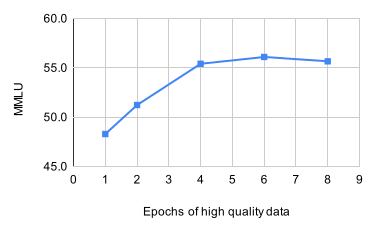
\includegraphics[width=0.95\textwidth]{figures/crawl_epoch.pdf}
    \\\vspace{-0.2\abovedisplayskip}
    \caption{MMLU accuracy (\%) vs. number of epochs of high-quality crawl in the data mix.}
    \label{fig:crawl_epoch}
\end{figure}


\paragraph{Quality Estimation of Other Datasets:}

We assess how our \ccderiv, papers, books and high quality datasets such as math, code and Wiki compare to \ccmq,\ccmhq and \cchq quality crawl data. 
%\cchq corresponds to \textit{High}-quality web crawl and \ccmq corresponds to the aggregate of \textit{Medium-High} and \textit{Medium}-quality web crawl from the previous discussion.
%\cchq corresponds to high quality scores 3 to 5 in Table \ref{table:crawl_data_mixing_percent}, while \ccmq corresponds to score 2. 
We continue training the last checkpoint of \phaseone-$\mathtt{Blend4}$, for an additional 50B tokens using a data mix that consisted $66$\% of the data being tested, mixed with $34$\% of \cchq. 




The results in Table \ref{tab:crawl++_papers_vs_crawl} show that \ccderiv, papers and books datasets have similar accuracies to \ccmhq on the majority of benchmarks, and lag behind \cchq. 
As such, we group them under the "medium-quality" data category for our experiments (see \S\ref{subsec:data_sources}). 
The high quality datasets have an average accuracy better than \cchq.








\subsection{Epoch-Based Analysis}
\label{subsec:epoch_results}

\begin{tcolorbox}[colframe=black!80, colback=gray!10, coltitle=white, title=Insights, fonttitle=\bfseries]
\begin{itemize}
\item We recommend 6 epochs of high-quality crawl and 8 epochs of math and task data for data mixing.
%\item Increasing the epochs of high-quality crawl, math, and task data improves performance to a certain point followed by degradation, highlighting the importance of balancing data quality with diversity to avoid overfitting.
%\item Optimal data exposure in training should consider the number of epochs, not just data quantity or proportions. Too many epochs of the same data can lead to diminishing returns. %Careful epoch-based tuning in data mixing for two-phase training is required.
%\kk{I feel like it is better to keep the 'insights' tight and short} \steven{just shortened, thoughts?}
\end{itemize}
\end{tcolorbox}

%We conducted further experiments to investigate how the weighted sampling of data mix should be done. 
We take the number of epochs of high quality datasets into account while creating our \phaseone and \phasetwo blends.
%We investigate the optimal number of epochs of high-quality data sources to be seen in pretraining before the downstream accuracy saturates.
We experiment with different numbers of epochs for high-quality crawl, math, and task data.

%We evaluated how the number of epochs of high-quality crawl tokens will affect the pretrained LLM's general understanding capability. 
Since, majority of web crawl is used in \phaseone, we pretrained an 8B model with 1T tokens, using different epochs of high-quality crawl tokens in the data mix, and evaluate each model's MMLU score. 
Note that we keep the overall percentage of web crawl the same in all the experiments.
As we can see in Figure~\ref{fig:crawl_epoch}, increasing the number of high-quality tokens increases the MMLU score until 6 epochs. 
We primarily present MMLU score because these experiments do not include high amount of math or code data.
%This demonstrates that seeing the same high-quality data too many times can hurt the model's performance. 
%This matches with our intuition, that we should find the proper balance between data quality and diversity to achieve better performance.



\begin{table}[t]%[h!]
\begin{center}
\scalebox{0.7}{\begin{tabular}{@{}lcrrrrr@{}}
\toprule
\textbf{Domain} & \textbf{Epochs} & \textbf{MMLU} & \textbf{Reason.} & \textbf{GSM8K} & \textbf{Code}	& \textbf{Avg.} \\
\toprule
Math & 1 & 57.06 & 60.51 & 36.47 & 33.55 & 51.49 \\
Math & 4 & 57.01 & 60.32 & 38.21 & 35.20 & 51.92 \\
Math & 8 & 56.58 & 60.18 & 37.98 & 37.01 & \textbf{52.28} \\
Math & 12 & 56.09 & 59.69 & 38.29 & 35.70 & 51.63 \\
\midrule
Task Data & 1 & 56.37 & 59.39 & 34.50 & 30.57 & 49.84 \\
Task Data & 4 & 56.57 & 59.46 & 40.18 & 35.27 & 51.53 \\
Task Data & 8 & 56.58 & 60.18 & 37.98 & 37.01 & \textbf{52.28} \\
Task Data & 12 & 56.77 & 59.96 & 38.44 & 36.04 & 51.93 \\
\bottomrule
\end{tabular}}
\end{center}
\caption[]{Results of varying the number of epochs of math and task data during \phasetwo of training.%\todo{modify caption as necessary} 
\label{tab:epoch-results}}
\end{table}


%We also investigate the optimal number of epochs for high-quality domains like math and task data.
Since, majority of math and task-data is seen in \phasetwo, Table~\ref{tab:epoch-results} presents results for different numbers of epochs for them in \phasetwo. 
%It illustrates that more epochs of math lead to diminishing performance on MMLU and reasoning, with unstable but generally increasing performance on GSM8K and Code. 
It shows that $\approx$ 8 epochs of math is a good balance while not sacrificing accuracy on MMLU and reasoning. 
For task data, all metrics generally improve with more epochs, although there appears to be diminishing returns on several past epoch 8. 
%Hence, sticking to $\approx$ 8 epochs of task data also seems to be a good balance. 
Note that 8 epochs of both math and task data corresponds to our best \ponebfourptwobone blend combo from \S\ref{subsec:two-phase-results}.
%Overall, we see that finding the optimal amount of a data source to include in our two-phase training blends should not rely entirely on absolute or relative amounts, but also on the number of epochs of the data, as over-exposure to the same data (too many epochs) can lead to diminishing returns.

%\todo{I helped finish the above section. Shrimai: double-check what I wrote.}

%\todo{Shrimai: explain more details of these expts. Firstly, is this during phase-2? Yes. For math and task, go with overall average to determine the best epoch. If so, what was the phase-1 blend/checkpoint? Phase-1-blend4, 1T total tokens. Also, the total number of tokens, LR decay strategy, size of each epoch, etc. How do the epoch results compare to simply using \% of the total data?}







%\steven{I feel as though the "crawl data mix", "epoch-based analysis", "scaling", and "how eval tasks evolve over time" sub-sections (4.6-4.9) are more detailed/extended analysis that are different from the main data mixture exps (4.1-4.5). Not sure if including everything here flows well, or is too overwhelming amount of info/results.}


%\todo{Where should we mention the best overall blend/approach? Basically combining phase-1 and phase-2 and all the different strategies we discuss in the previous section. Also, we should make sure the best overall blend/approach is consistent with the individual results (e.g. best phase1 and phase2 blends).}


\subsection{Optimal Duration of Phase-2}
\label{subsec:pct-upsampling}

\begin{tcolorbox}[colframe=black!80, colback=gray!10, coltitle=white, title=Insights, fonttitle=\bfseries]
\begin{itemize}
\item Pretraining with the \phasetwo blend for the final 40\% gives the best results.
%\item Higher upsampling generally improves performance up to a certain point, especially in math and code tasks.
%\item $\approx$ 40\% upsampling appears to be optimal, yielding peak performance on difficult benchmarks without compromising generalization. %\item Overfitting occurs past this point, indicating that over-extending \phasetwo training can be detrimental.
\end{itemize}
\end{tcolorbox}

We investigate the percentage of phase-2 to use in the whole pretraining regime. 
We experiment with 0 to 50\% of \phasetwo in the whole of pretraining.
%ranging from the last 5\% of training up to the last 50\% of training. 
The longer the duration of \phasetwo, the shorter the duration of \phaseone.
%as the earlier we switch to \phasetwo training. 
We use the \ponebfourptwobone blend combination that we found best in \S\ref{subsec:two-phase-results}.


Table \ref{tab:data-upsampling-results-2} illustrates that a higher percentage of \phasetwo until 40\% is better overall, especially in math and code.
%although MMLU and reasoning slightly fluctuate around the same numbers. 
Going above this, e.g. to \phasetwo as 50\% of training, downstream accuracies start to degrade across the board, potentially due to overfitting. 
%It seems that $\approx$ 40\% of upsampling is a good stopping point, where performance on challenging benchmarks peaks without hurting generalization. %before gains start to saturate on GSM8K and code, potentially due to overfitting.
%Hence, we use 30\% upsampling (switch from \phaseone to \phasetwo after 70\% of training) for our final two-phase experiments discussed in Section \ref{subsec:two-phase-results}.%\todo{This is based on my original phase 2 upsampling exps. likely need to change based on Shrimai and Kezhi's new exps. However, hope it's consistent with my results.}
%\shrimai{Write up about Table 8}



% \begin{table}[t]%[h!]
% \begin{center}
% \scalebox{0.75}{\begin{tabular}{@{}lrrrrr@{}}
% \toprule
% \textbf{Upsampling \%} & \textbf{MMLU} & \textbf{Reason.} & \textbf{GSM8K} & \textbf{Code}	& \textbf{Avg.} \\
% \toprule
% $0$ & 56.10 & 61.81 & 16.60 & 16.22 & 37.68\\
% %$5$ & 56.25 & 62.03 & 18.50 & 21.31 & 39.52\\
% $10$ & 56.33 & 61.78 & 22.59 & 21.53 & 40.56\\
% $20$ & 55.78 & 61.94 & 27.82 & 22.11 & 41.91\\
% $30$ & 56.01 & 61.22 & 31.39 & 22.80 & 42.85\\
% $38$ & 55.97 & 60.87 & 33.06 & 23.70 & 43.40\\
% \bottomrule
% \end{tabular}}
% \end{center}
% \caption[]{Results of different upsampling \% (duration of \phasetwo) using $\mathrm{B}_{1C}$ and $\mathrm{B}_{2C}$.
% \label{tab:data-upsampling-results}}
% \end{table}


\begin{table}[t]%[h!]
\begin{center}
\scalebox{0.75}{\begin{tabular}{@{}lrrrrr@{}}
\toprule
\textbf{\phasetwo \%} & \textbf{MMLU} & \textbf{Reason.} & \textbf{GSM8K} & \textbf{Code}	& \textbf{Avg.} \\
\toprule
$0$ & 56.10 & 61.81 & 16.60 & 16.22 & 37.68 \\
$10$ & 56.52 & 59.70 & 33.13 & 32.55 & 50.48 \\
$20$ & 56.54 & 59.93 & 40.16 & 34.29 & 51.58 \\
$30$ & 56.58 & 60.18 & 37.98 & 37.01 & 52.28 \\
$40$ & 56.28 & 60.34 & 40.33 & 38.33 & \textbf{52.86} \\
$50$ & 55.94 & 59.82 & 37.68 & 36.86 & 51.96 \\
\bottomrule
\end{tabular}}
\end{center}
\caption[]{Results of different durations of \phasetwo using \ponebfourptwobone. 
\label{tab:data-upsampling-results-2}}
\end{table}


\section{Related Work}
%\begin{itemize}
    %\item Data selection \& mixture work
    %\item Upsampling \& annealing work
    %\item Curriculum work (including babyLM curriculum work like Steven's and babyview)
    %\item Examples: Llama, OLMo, Doremi, Data Data everywhere, FineWeb Datasets, Reuse Don’t Retrain, DataComp-LM, Does your data spark joy?, The Pile, Dolma, Curriculum learning survey, Continual learning of LLMs survey, etc.
    %\item Group the above papers into appropriate categories
%\end{itemize}

%To train effective LLM, some research has recently focused on the selection, composition, and ordering of training data. This section summarizes key contributions in three areas.

Selecting and structuring pretraining datasets is important to improve model generalization and efficiency.
%Works like \citet{llama3-dubey2024llama3herdmodels,olmo-groeneveld-etal-2024-olmo,together2023redpajama} focus on open-source availability, with 
\citet{llama3-dubey2024llama3herdmodels} emphasize openness and accessibility of models, \citet{together2023redpajama,soldaini-etal-2024-dolma} assemble an open corpus of trillions of tokens for large-scale training, and \citet{olmo-groeneveld-etal-2024-olmo} release a truly Open Language Model, including its framework, training data, and code. 
%\citet{gao2020pile800gbdatasetdiverse} emphasize diversity, aiming to balance domains within large datasets to enhance the adaptability of LLM across various contexts. 
Studies such as \citet{li2024datacomplm,fineweb-penedo2024the} demonstrating that refined data selection impacts model accuracies more significantly than simply the quantity of data. 
But these studies are primarily aimed at CC data and they do not suggest any data mixing strategies for pretraining.
\citet{parmar-etal-2024-data} provide a systematic approach to building effective LLM pretraining datasets with ablations on data attributes, and existing curation, selection, and sampling methods. 
In our work, we provide a systematic approach to craft data blends and to order the data in pretraining.
%, and also analyze attributes to optimize data selection. %(English, multilingual, and code). The authors analyze attributes such as quality, toxicity, and domain to optimize data composition, aiming to improve model performance and present an actionable framework for dataset development. %These contributions illustrate the ongoing focus on data quality over quantity, shaping the construction of next-generation pretraining datasets.

Strategic weighting and timing of data usage can also noticeably impact model accuracies. 
Techniques like domain upsampling \cite{domain-upsampling-blakeney2024doesdatasparkjoy,llama3-dubey2024llama3herdmodels} towards the end of training have been shown to be effective.
\citet{snowflake-arctic,olmo-groeneveld-etal-2024-olmo} provide details about high level blends for their pretraining process.
In contrast, our work provides fine grained details about the data blend creation process along with actionable steps that model developers can use to develop data blends and order.
Prior work \cite{shen2023slimpajama,longpre2024pretrainer,pmlr-v162-mindermann22a,doremi-NEURIPS2023_dcba6be9,xie2023data,shao2024balanced} investigates optimizing data mixtures based on clustering methods, manually designed domain composition weights, proxy models or reference models to determine data composition weights and sample-level data selection. 
Our work primarily focuses on data ordering and scaling of data blends in pretraining and can be used in conjunction with other data sampling techniques.
%\citet{parmar2024reusedontretrainrecipe} examine how to effectively design data distributions and learning rate schedules for the continued pretraining of LLM.%Studies on scaling laws for neural language models highlight how upsampling and careful tuning of data composition can offset diminishing returns at scale. %Together, these works underline the efficacy of upsampling and annealing strategies in refining language models during training.

Curriculum learning approaches inspired by human learning offer an ordered way to introduce data gradually to enhance model learning. 
%\citet{curriculum-survey} outline its broad applicability across machine learning, including different domains and tasks, and the challenges and potential solutions for designing effective curricula. %They also discuss some particular curriculum strategies for language models including easy-to-hard and task progression. %, from general LLM to task-specific tuning.
%In the context of BabyLM \cite{conll-2023-babylm}, 
\citet{martinez-etal-2023-climb,curriculum-survey,feng-etal-2024-child} investigate cognitively-motivated curriculum-based training including vocabulary, and objective curricula, and outline and the challenges and potential solutions for designing effective curricula. 
%examine the impact of global developmental ordering of child-directed speech on model learning, but find no noticeable impact. 
Our work shows that ordering of data based on quality in pretraining LLMs has a significant impact of downstream accuracies.
%These works highlight that %, depending on the domain, model architecture, data scale and content, and downstream tasks,
%ordered exposure to data can potentially affect model accuracy and generalization, but sometimes shows limited to no impact.
%\todo{steven: add citations later}%. data data everywhere, olmo, reuse don't retrain}
%\todo{steven: read https://arxiv.org/pdf/2402.14526v1}

%\section{Conclusion \& Future Work}
\section{Conclusion}
%\begin{itemize}
    %\item Discuss/summarize our research questions, high-level approach, and the major results/takeaways
    %\item Similar to abstract
    %\item Then, discuss remaining challenges \& potential future work directions
    %\item Can include investigations of the impact of domain upsampling on long-term robustness (e.g. overfitting) and bias \& fairness, applications to niche or language-specific models, and applications to multimodal models
%\end{itemize}
%\mostofa{remove performance throughout the paper}
In conclusion, through extensive experiments, we demonstrate the effectiveness of a two-phase pretraining approach for LLM. %, especially when high-quality data is emphasized near the end of training. We find that phase-two  %paired with cosine annealing to a low learning rate, 
For the initial training phase, a more general data distribution consisting of mainly of web crawl proves most effective, while phase two benefits from a comprehensive data blend, with additional focus on math, code, and task data. Phase-two for the last $\approx$40\% of training yields the best results, and over-extending it leads to diminishing returns. Increasing model size and token horizon further enhances accuracy, demonstrating the scalability of our approach. Importantly, we also show that considering both the quality of the data (including web crawl) and the number of epochs of each data source is crucial to attain optimal results and prevent overfitting.
%Importantly, we also show that preventing overfitting requires considering not only data proportions but also the number of epochs of high-quality data in each phase.
%Overall, our findings suggest that a well-structured two-phase training approach, with careful data selection and management, is essential for optimizing LLM performance while maintaining scalability and robustness across downstream tasks.
%Overall, our findings underscore the value of a well-structured two-phase training framework with domain upsampling, where balanced data quality and diversity drive optimal LLM performance, robustness, and scalability.

\begin{comment}
    Future work can investigate potential effects of two-phase training other than overfitting, e.g. impacts on bias \& fairness. Further, it would be interesting to see how two-phase training can be applied to niche domains or applications, e.g. medicine or finance, %or other languages (other than English).\footnote{While we include multilingual data in part of our training, it is a limited amount, and our downstream tasks are in English.\todo{double-check this.}} 
or a multimodal setting, e.g. vision-language models (VLM). 
%Lastly, the exploration of two-phase training for smaller scales, e.g. BabyLM, could be  another fruitful direction.
\end{comment}


\section*{Limitations}

%1. multi-phase, order of phases. more architectures, evaluation metrics (e.g. ToM and psych-inspired, analogical reasoning), 

Some limitations of our work include our present suite of models and evaluation benchmarks. 
We can extend our work and show the effectiveness of two-phase pretraining approach on more LLM architectures such as Mamba~\cite{gu2023mamba}, other hybrid SSM based architectures~\cite{glorioso2024zamba,lieber2024jamba} and mixture of experts~\cite{shazeer2017outrageously}. %including LLama-3.
While our evaluation benchmarks are quite comprehensive, we could potentially expand to an even broader range of evaluations, including nuanced domain-specific or interactive tasks, or more theory of mind and developmental psychology-inspired benchmarks. 
This includes assessing capabilities such as analogical reasoning \cite{webb2023emergentanalogicalreasoninglarge}.
Further, our scaling experiments could be expanded. Scaling up to hundreds of billions of parameters or significantly longer training may yield additional insights. Lastly, while our work focuses on two-phase training and shows its efficacy, we can potentially investigate multi-phase training, and the impact of the order of the phases. However, we believe this is more suited for future work. Overall, these are directions to potentially improve and expand upon our work. 
Despite these potential limitations, we feel that our current work is an insightful and useful contribution to the research community.

\section*{Ethical Considerations}

%The majority of our datasets and evaluation benchmarks are already existing, publicly available datasets and benchmarks, intended for public use.

Our research uses publicly available and commonly used datasets in LLM development. %in the development of LLM.
These sources, including Common Crawl, Wikipedia, and code repositories, are widely adopted in the research community. We examined the quality and origins of our data, prioritizing high-quality, domain-relevant data sources to improve LLM capabilities in a responsible manner. However, web crawl data may inherently contain biases or inappropriate content despite filtering efforts. We used established data cleaning and quality assurance procedures but acknowledge that potential biases may persist and impact model behavior in certain circumstances.

%Further, the Megatron models we train on our data are safe and controlled language models, with a low risk of offensive content. %We also manually examined a large subset of the data and ensured there were no ethical issues. This includes profanities, racism, bias, offensive words, and other malicious language.

We recognize that scaling models and exploring data blending strategies require significant computational resources, which may raise environmental concerns. To mitigate this, we focused on efficient training strategies, such as two-phase training, to improve accuracy without excessively increasing resource usage. Future studies could benefit from exploring energy-efficient training methods to further minimize the environmental impact. %of LLM research.

%We acknowledge the potential weaknesses of our trained models. We will never use or encourage their use for real-world purposes. Our initial experiments are conducted purely for investigation purposes to test our hypotheses. 

Our models, data blends, and accompanying publication are intended solely for research purposes, with no intended real-world application without additional safety evaluations. We caution against deploying models based on our methods without thorough testing, as they may carry unknown risks, particularly when applied to tasks involving sensitive or personal information. Our work aims to advance the understanding of LLM training strategies, and we feel that it is an important contribution to the research community. We encourage researchers to expand upon our work while further investigating the ethical and societal implications of LLM.

%Our models, datasets and mixtures, and accompanying publication are intended only for research purposes and to assess the effectiveness of two-phase training for LLM. We do not foresee any explicit way that malicious actors could specifically misuse our trained models or models that could be trained on our dataset.

%\section*{Acknowledgments}

% Bibliography entries for the entire Anthology, followed by custom entries
%\bibliography{anthology,custom}
% Custom bibliography entries only
\bibliography{custom}

\newpage
\appendix

\section{Model Specifications}
\label{app:detailed_model_specs}

We use RoPE position embeddings \cite{rope-paper}, RMSNorm layer normalization \cite{RMSNorm}, with Grouped Query Attention \cite{ainslie-etal-2023-gqa}. The maximum sequence length is 4096. We use a global batch size of 1536, 
and the Adam optimizer \cite{kingma2017adammethodstochasticoptimization} with $\beta=(0.9,0.95)$ and $\epsilon=1e$-$08$. 

\phaseone training uses cosine $LR$ decay with an initial $LR$ of $3e$-$4$ and targeted to reach a min-$LR$ of $3e$-$6$ at the end of the full training run (both phases). 
We start \phasetwo with the intermediate $LR$ reached at the end of \phaseone, and anneal using cosine $LR$ decay to $3e$-$6$ (\S\ref{app:lr_schedule}). 
Our experiments are run using up to 1024 NVIDIA H100 GPUs.

\section{Detailed Two-Phase Pretraining Results (Reasoning, MMLU, Code)}
\label{app:detailed_exp_results}

Tables \ref{tab:P2-eval-results-reasoning} to \ref{tab:model-scaling-eval-results-MMLU-code} contain detailed evaluation results of the major experiments reported in \S\ref{subsec:two-phase-results} for reasoning, MMLU, and code, broken down by individual categories and benchmarks. They correspond to the results found in Tables \ref{tab:phase2-results} to \ref{tab:25B-results} in \S\ref{subsec:two-phase-results}.



Table~\ref{tab:phase2-blend6} shows the comparison of $\mathtt{Blend1}$ and $\mathtt{Blend6}$ used in scaling experiments in Table~\ref{tab:1.7T-results}.
If we use the same $\mathtt{Blend1}$ as is and train for more number of tokens (1.7T) then the number of epochs seen of each dataset would be higher compared to 1T training.


\begin{table}[t]%[h!]
\begin{center}
\scalebox{0.65}{\begin{tabular}{@{}llrr@{}}
\toprule
\textbf{Category} & \textbf{Domain} & \textbf{Blend1} & \textbf{Blend6} \\
\toprule
Web Crawl & - & 31.0 & 49.0 \\
\midrule
\multirow{3}{*}{High Quality} & Math & 24.0 &  14.4 \\
& Wiki & 1.0 & 0.6 \\
& Code & 20.0 & 12.0 \\
\midrule
\multirow{3}{*}{Medium Quality} & Books & 8.0 & 8.0 \\
& Papers & 4.0 & 4.0 \\
& \ccderiv & 7.0 & 7.0 \\
\midrule
Multilingual & - & 3.7 & 4.2 \\
\midrule
Task Data & - & 1.3 & 0.8\\
\bottomrule
\end{tabular}}
\end{center}
\caption[]{Comparison of $\mathtt{Blend1}$ and $\mathtt{Blend6}$ (in \%) used for scaling the token budget in \S\ref{subsec:scaling_results} and Table \ref{tab:1.7T-results}.
\label{tab:phase2-blend6}}
\end{table}



\section{Details of Quality-Based Data Blend}
\label{app:quality-based-blend}
%\todo{Where do we actually refer to this in the main paper?}

\begin{table}[h]
\small
\centering
\resizebox{0.6\textwidth}{!}{%
\begin{tabular}{lrr}
\toprule
\textbf{Quality Label} & \textbf{ND} & \textbf{WS} \\
\midrule
High & 0.01 & 0.04 \\
Medium-High & 1.08 & 6.42 \\
Medium & 7.01 & 41.83 \\
Medium-Low & 26.46 & 25.09 \\
Low & 64.44 & 0.00 \\
%Low & 59.05 & 0.00 \\
%Low-Low & 6.39 & 0.00 \\ 
\bottomrule
\end{tabular}%
}
\caption{Data blends for CC Quality estimation experiment. The overall percentage of the Common Crawl Snapshots in our experiments is fixed at 73.3\%.}
\label{table:crawl_data_mixing_percent}
\end{table}


We first compare a baseline blend (ND) which uses the natural distribution of tokens with a smartly constructed weighted sampling blend (WS).
ND is based on the number of tokens that belong in each category as opposed to utilizing the quality label 
%and upsampling certain categories of tokens, 
i.e. if 59\% of the tokens belong to \textit{Low} then 59\% of tokens seen during pretraining would belong to \textit{Low}.
We then create a data blend (WS) based on weighted sampling of high and medium-quality tokens.
The idea is to upsample high and medium-quality crawl documents and not use the low-quality data at all.
Table~\ref{table:crawl_data_mixing_percent} shows the token percentages that belong to each of the five quality labels for both ND and WS blends.
Table~\ref{table: crawl_data_mixing_comp} illustrates the results of the two models trained on the ND and WS data blends of web crawl, respectively. 
%comparison results of using our weighted sampling way with using random sampling data mixing over high-quality pretraining tokens are shown in Table \ref{table: crawl_data_mixing_comp}. 
We see that our data blend (WS) outperforms on most of the evaluation tasks by a large margin, and the improvement on MMLU is substantial. %on both datasets.

\begin{table}[]
\centering
\resizebox{\textwidth}{!}{%
\begin{tabular}{lcccc}
\toprule
\textbf{Data Mixing} & \textbf{MMLU} & \textbf{Reason.} & \textbf{GSM8K} & \textbf{Code} \\
\midrule
ND & 42.94 & 59.40 & 8.11 & 19.25 \\
WS & 56.10 & 61.60 & 11.98 & 17.41 \\
\bottomrule
\end{tabular}%
}
\caption{Our \textit{WS}: weighted sampling data mixing method outperforms the \textit{ND}: natural distribution method.}
\label{table: crawl_data_mixing_comp}
\end{table}


\section{Finegrained \phasetwo Blend Experiments}
\label{app:finegrained_upsampling_exps}


% \begin{tcolorbox}[colframe=black!80, colback=gray!10, coltitle=white, title=Insights, fonttitle=\bfseries]
% \begin{itemize}
% \item %\textbf{Crawl, Math, \& Code:}
% A comprehensive data blend containing task data and higher proportions of code and math data in \phasetwo leads to higher downstream accuracy.
% %\item %\textbf{Task Data:}
% %Task data (e.g. FLAN \& synthetic GSM8K) improves performance. % on challenging tasks without harming other benchmarks.
% %\item %\textbf{Coding Languages, Books, Patents, \& Papers:}
% %Including all coding languages, books, patents, and papers data is preferable, as removing specific datasets yields minimal or negative impacts.
% %\item %\textbf{All Data Mixture:}
% %A comprehensive mix of all data sources %(including FLAN, GSM8K, math, code)
% %is best overall.
% \end{itemize}
% \end{tcolorbox}

We investigate fine-grained \phasetwo blends to determine the optimal blend.
%to determine the best domain upsampling data blend during \phasetwo of training. 
%Specifically, different data blends $\mathrm{B}_{2}$, including which domains and their percentages in the final blend. 
For these experiments, we use a model trained on a \phaseone blend for 900B tokens (10\% \phasetwo duration), with a linear $LR$ decay to $0$. % the control data mix for \phaseone, $\mathrm{B}_{1C}$, shown in Figure \ref{fig:P1_control_pie-chart} in \S\ref{app:pie_charts}. 


\paragraph{Crawl, Math, \& Code:} We investigate different percentages of high-quality crawl, math, and code data as shown in Table~\ref{tab:phase2-finegrained-blends}. 
%Upsampling commonly involves training on higher amounts of high-quality specialized data such as math and code, but what amounts should be used? 
%We investigate this by trying a few different blends of crawl (high-quality subset, see Section \ref{subsec:crawl_data_mix}), math, and code data, found in Table \ref{tab:phase2-finegrained-blends}. 
Table \ref{tab:phase2-finegrained-results} demonstrates that a higher amount of math data (i.e. 30\%) helps across the board. 
However, code data results are mixed, as too much code without enough math ($\mathtt{CMC}$-$\mathtt{B1}$) seems to hurt all non-code metrics. Comparing ($\mathtt{CMC}$-$\mathtt{B2}$) vs. ($\mathtt{CMC}$-$\mathtt{B3}$), more than 15\% code does not add as much value, as gains saturate. Trading off crawl data for more code data also slightly hurts MMLU. %, and surprisingly, coding tasks.
As such, we decide that a final blend consisting of a higher amount of crawl and math with a moderate amount of code seems best overall. This corresponds to $\mathtt{CMC}$-$\mathtt{B3}$ in Table \ref{tab:phase2-finegrained-blends}, which consists of 30\% crawl, 33\% math, and 15\% code. 
%This is the same control blend for \phasetwo, $\mathrm{B}_{2C}$, that we use for several experiments in Sections \ref{subsec:lr_schedule} and \ref{subsec:pct-upsampling}.

\paragraph{Task Data:} Second, we investigate the inclusion of task data. Specifically, adding FLAN and synthetically-generated GSM8K-train data (similar to data augmentation approaches \cite{feng-etal-2021-survey}) to the $\mathtt{CMC}$-$\mathtt{B3}$ blend. 
Our FLAN data consists of a mixture of normal FLAN and FLAN-CoT (chain-of-thought) data. 
%We feel that chain-of-thought training data may further help with more challenging tasks such as GSM8K-train. 
%\steven{we don't actually test this out empirically (e.g. FLAN vs. FLAN-CoT) so not sure if we should say this.} 
%We only have $\approx$ 300M tokens of FLAN data, so we try lower proportions of FLAN corresponding to 10 and 20 epochs. 
We compare 10 and 20 epochs of FLAN. 
These blends can be found in Table \ref{tab:phase2-finegrained-blends-pt2}, with the results in Table \ref{tab:phase2-finegrained-results}. We can see that including synthetic GSM8K-train and FLAN data noticeably improves GSM8K scores while not detrimenting the other benchmarks. In fact, FLAN data also helps further improve MMLU and reasoning. 20 epochs of FLAN seems better than 10 epochs overall. Hence, including task data for \phasetwo of training seems to be a good idea.

\paragraph{All Data Mixture:} Lastly, we investigate a final \phasetwo data mixture which is a combination of all the data sources we tried, including FLAN, GSM8K, and relatively higher amounts of math and code data. For this experiment, we use 30\% upsampling with $LR$ cosine decay to $3e-6$. This blend can be found in Table \ref{tab:phase2-finegrained-blends-pt2}, with the results at the bottom of Table \ref{tab:phase2-finegrained-results}.\footnote{The $\mathtt{CMC}$-$\mathtt{Blend3}$-$30\%$ result at the bottom of Table \ref{tab:phase2-finegrained-results} is also using 30\% upsampling with $LR$ cosine decay to $3e-6$.} We find that mixing all data sources %noticeably improves non-MMLU results, while MMLU remains relatively stable.
helps greatly with GSM8K, noticeably with coding and reasoning, while retaining accuracy on MMLU. Hence, the final \phasetwo blends we investigate in \S\ref{subsec:two-phase-results} (Table \ref{tab:phase2-blends}) are motivated by these ablations -- they are blends of all data sources, including task data, with higher proportions of math and code.

\section{Annealing Learning Rate Schedule}
\label{app:lr_schedule}

We investigate different learning rate ($LR$) schedules for phase \phasetwo. 
Specifically, using the same \phasetwo blend for a 10\% duration, 
%(the last 10\% of training tokens are \phasetwo)
we try different $LR$ strategies. 
We compare cosine vs. linear $LR$ decay functions, and also compare decaying to a final $LR$ of $0$ vs. $3e$-$6$ (1\% of the original \phaseone starting $LR$ of $3e$-$4$). 
Not decaying $LR$ entirely to 0 leaves room for post-training, which is likely preferable. 

As seen in Table \ref{tab:LR-anneal-results}, there is a negligible difference between linear and cosine $LR$ decay, so we choose cosine decay for consistency with \phaseone.
We also see that $LR$ decay to $3e$-$6$ is comparable to decaying all the way to $0$, while leaving room for post-training. 
Hence, our final chosen annealing strategy is cosine $LR$ decay to $3e$-$6$, which we use for our final two-phase experiments in \S\ref{subsec:two-phase-results}.





\begin{table*}[t]%[h!]
\begin{center}
\scalebox{0.66}{\begin{tabular}{@{}lccccccccc@{}}
\toprule
\textbf{Exp.} & \textbf{ARC-Easy} & \textbf{ARC-Challenge} & \textbf{RACE} & \textbf{PIQA} & \textbf{WinoGrande} & \textbf{HellaSwag} & \textbf{OpenBookQA} & \textbf{CommonsenseQA} & \textbf{Avg.}\\
\toprule
\phaseone-$\mathtt{Blend1}$ & 75.97 & 51.19 & 36.36 & 80.96 & 67.64 & 76.23 & 44.00 & 53.07 & 59.12 \\
\phaseone-$\mathtt{Blend4}$ & 77.23 & 53.24 & 36.46 & 80.47 & 68.35 & 76.48 & 44.40 & 53.15 & 59.54 \\
\midrule
\poneboneptwobone & 78.32 & 51.54 & 36.75 & 79.76 & 66.54 & 76.44 & 43.80 & 61.67 & 60.04\\
\poneboneptwobtwo & 78.79 & 53.07 & 35.69 & 80.79 & 67.09 & 76.52 & 43.40 & 61.18 & 60.15\\
\poneboneptwobthree & 79.29 & 53.16 & 36.27 & 79.76 & 66.77 & 76.43 & 42.80 & 61.43 & 60.08 \\
\poneboneptwobfour & 78.37 & 52.99 & 36.65 & 80.30 & 66.93 & 76.67 & 43.80 & 61.92 & 60.26 \\
\poneboneptwofive & 79.21 & 52.56 & 36.75 & 80.63 & 67.25 & 76.64 & 44.00 & 61.83 & 60.41 \\
\textbf{\ponebfourptwobone} & 80.30 & 54.95 & 35.50 & 79.98 & 68.35 & 76.55 & 43.80 & 56.59 & 60.18 \\
\ponebfourptwobtwo & 79.92 & 54.10 & 35.50 & 80.20 & 67.96 & 76.75 & 43.80 & 56.35 & 60.00 \\
\ponebfourptwobthree & 79.92 & 54.27 & 35.12 & 80.20 & 67.56 & 76.39 & 44.20 & 57.08 & 60.08 \\
\ponebfourptwobfour & 79.92 & 54.27 & 35.89 & 80.47 & 67.25 & 76.79 & 43.80 & 56.18 & 59.98 \\
\ponebfourptwobfive & 79.29 & 54.44 & 37.03 & 79.98 & 67.80 & 76.92 & 44.80 & 57.41 & 60.35 \\
\bottomrule
\end{tabular}}
\end{center}
\caption[]{Final reasoning evaluation results after \phasetwo of training, broken down by individual benchmark. Corresponds to Table \ref{tab:phase2-results} in \S\ref{subsec:two-phase-results}.
\label{tab:P2-eval-results-reasoning}}
\end{table*}

\begin{table*}[t]
\begin{center}
\scalebox{0.70}{\begin{tabular}{@{}lcccccccccc@{}}
\toprule
\textbf{Exp.} & \multicolumn{5}{c}{\textbf{MMLU}} & \multicolumn{5}{c}{\textbf{Code}} \\
\cmidrule(lr){2-6} \cmidrule(lr){7-11}
 & \textbf{STEM} & \textbf{Humanities} & \textbf{Social Sciences} & \textbf{Others} & \textbf{Avg.} & \textbf{HumanEval} & \textbf{HumanEval+} & \textbf{MBPP} & \textbf{MBPP+} & \textbf{Avg.} \\
\toprule
\phaseone-$\mathtt{Blend1}$ & 45.61 & 50.24 & 65.29 & 61.54 & 55.00 & 18.90 & 13.41 & 31.52 & 30.42 & 23.56 \\
\phaseone-$\mathtt{Blend4}$ & 48.30 & 49.88 & 67.53 & 62.79 & 56.25 & 18.90 & 16.46 & 42.80 & 32.28 & 27.61 \\
\midrule
\poneboneptwobone & 47.57 & 51.12 & 65.88 & 62.34 & 56.04 & 32.32 & 27.44 & 42.41 & 42.59 & 36.19 \\
\poneboneptwobtwo & 48.65 & 50.41 & 65.78 & 61.67 & 55.88 & 31.71 & 26.83 & 42.41 & 42.59 & 35.89 \\
\poneboneptwobthree & 47.61 & 50.69 & 65.78 & 61.96 & 55.80 & 31.10 & 25.61 & 43.97 & 42.33 & 35.75 \\
\poneboneptwobfour & 48.11 & 50.84 & 65.81 & 62.76 & 56.15 & 28.66 & 25.61 & 42.80 & 42.86 & 35.59 \\
\poneboneptwofive & 48.94 & 51.41 & 66.14 & 62.28 & 56.49 & 28.66 & 23.78 & 42.02 & 43.12 & 34.40 \\
\ponebfourptwobone & 49.29 & 50.35 & 67.44 & 62.66 & 56.58 & 31.10 & 24.39 & 49.42 & 43.12 & 37.01 \\
\ponebfourptwobtwo & 49.44 & 50.92 & 67.47 & 62.99 & 56.89 & 30.49 & 25.00 & 49.81 & 42.59 & 36.97 \\
\ponebfourptwobthree & 49.19 & 49.37 & 66.88 & 62.60 & 56.10 & 27.44 & 20.73 & 48.25 & 44.18 & 36.15 \\
\ponebfourptwobfour & 49.16 & 50.84 & 68.35 & 63.18 & 57.03 & 31.71 & 23.17 & 47.47 & 42.86 & 36.30 \\
\ponebfourptwobfive & 49.38 & 50.86 & 68.18 & 62.60 & 56.92 & 28.66 & 20.12 & 45.53 & 43.92 & 34.56 \\
\bottomrule
\end{tabular}}
\end{center}
\caption[]{Final MMLU and code evaluation results after \phasetwo of training, broken down by individual category/benchmark. Corresponds to Table \ref{tab:phase2-results} in \S\ref{subsec:two-phase-results}.
\label{tab:P2-eval-results-MMLU-code}}
\end{table*}


\begin{table*}[t]%[h!]
\begin{center}
\scalebox{0.71}{\begin{tabular}{@{}lccccccccc@{}}
\toprule
\textbf{Exp.} & \textbf{ARC-Easy} & \textbf{ARC-Challenge} & \textbf{RACE} & \textbf{PIQA} & \textbf{WinoGrande} & \textbf{HellaSwag} & \textbf{OpenBookQA} & \textbf{CommonsenseQA} & \textbf{Avg.}\\
\toprule
BASE & 78.75 & 53.84 & 35.69 & 80.30 & 68.51 & 76.30 & 45.40 & 51.68 & 59.69 \\
Two-Phase & 80.30 & 54.95 & 35.50 & 79.98 & 68.35 & 76.55 & 43.80 & 56.59 & 60.18 \\
\bottomrule
\end{tabular}}
\end{center}
\caption[]{Reasoning evaluation results of our two-phase training approach with \ponebfourptwobone vs. a randomized mixture of both blends across the entire 1T token training run, broken down by individual benchmark. Corresponds to Table \ref{tab:rand-vs-two-phase-result} in \S\ref{subsec:two-phase-results}.
\label{tab:random-BL-eval-results-reasoning}}
\end{table*}

\begin{table*}[t]
\begin{center}
\scalebox{0.72}{\begin{tabular}{@{}lcccccccccc@{}}
\toprule
\textbf{Exp.} & \multicolumn{5}{c}{\textbf{MMLU}} & \multicolumn{5}{c}{\textbf{Code}} \\
\cmidrule(lr){2-6} \cmidrule(lr){7-11}
 & \textbf{STEM} & \textbf{Humanities} & \textbf{Social Sciences} & \textbf{Others} & \textbf{Avg.} & \textbf{HumanEval} & \textbf{HumanEval+} & \textbf{MBPP} & \textbf{MBPP+} & \textbf{Avg.} \\
\toprule
BASE & 50.40 & 49.67 & 66.49 & 63.08 & 56.49 & 28.66 & 25.00 & 44.36 & 44.18 & 35.55 \\
Two-Phase & 49.29 & 50.35 & 67.44 & 62.66 & 56.58 & 31.10 & 24.39 & 49.42 & 43.12 & 37.01 \\
\bottomrule
\end{tabular}}
\end{center}
\caption[]{MMLU and code evaluation results of our two-phase training approach with \ponebfourptwobone vs. a randomized mixture of both blends across the entire 1T token training run, broken down by individual category/benchmark. Corresponds to Table \ref{tab:rand-vs-two-phase-result} in \S\ref{subsec:two-phase-results}.
\label{tab:random-BL-eval-results-MMLU-code}}
\end{table*}

\clearpage
\begin{table*}[t]%[h!]
\begin{center}
\scalebox{0.64}{\begin{tabular}{@{}llccccccccc@{}}
\toprule
\textbf{Exp.} & \textbf{Tok.} & \textbf{ARC-Easy} & \textbf{ARC-Challenge} & \textbf{RACE} & \textbf{PIQA} & \textbf{WinoGrande} & \textbf{HellaSwag} & \textbf{OpenBookQA} & \textbf{CommonsenseQA} & \textbf{Avg.}\\
\toprule
\ponebfourptwobone & 1T & 80.30 & 54.95 & 35.50 & 79.98 & 68.35 & 76.55 & 43.80 & 56.59 & 60.18 \\
\ponebfourptwobone & 1.7T & 79.84 & 52.90 & 36.27 & 79.65 & 70.01 & 77.79 & 44.80 & 61.75 & 60.88 \\
\ponebfourptwobsix & 1.7T & 80.09 & 55.29 & 37.03 & 80.79 & 70.09 & 78.53 & 46.00 & 60.85 & 61.63 \\
\bottomrule
\end{tabular}}
\end{center}
\caption[]{Reasoning evaluation results of scaling for 1.7T tokens vs. 1T tokens, with and without high-quality data epoch adjustment, broken down by individual benchmark. Corresponds to Table \ref{tab:1.7T-results} in \S\ref{subsec:two-phase-results}.
\label{tab:token-scaling-eval-results-reasoning}}
\end{table*}

\begin{table*}[t]
\begin{center}
\scalebox{0.67}{\begin{tabular}{@{}llcccccccccc@{}}
\toprule
\textbf{Exp.} & \textbf{Tok.} & \multicolumn{5}{c}{\textbf{MMLU}} & \multicolumn{5}{c}{\textbf{Code}} \\
\cmidrule(lr){3-7} \cmidrule(lr){8-12}
 & & \textbf{STEM} & \textbf{Humanities} & \textbf{Social Sciences} & \textbf{Others} & \textbf{Avg.} & \textbf{HumanEval} & \textbf{HumanEval+} & \textbf{MBPP} & \textbf{MBPP+} & \textbf{Avg.} \\
\toprule
\ponebfourptwobone & 1T & 49.29 & 50.35 & 67.44 & 62.66 & 56.58 & 31.10 & 24.39 & 49.42 & 43.12 & 37.01 \\
\ponebfourptwobone & 1.7T & 51.22 & 52.41 & 68.74 & 65.47 & 58.61 & 31.10 & 25.61 & 48.25 & 45.50 & 37.62 \\
\ponebfourptwobsix & 1.7T & 52.39 & 53.41 & 70.20 & 66.91 & 59.85 & 37.20 & 28.66 & 47.08 & 45.50 & 39.61 \\
\bottomrule
\end{tabular}}
\end{center}
\caption[]{MMLU and code evaluation results of scaling for 1.7T tokens vs. 1T tokens, with and without high-quality data epoch adjustment, broken down by individual category/benchmark. Corresponds to Table \ref{tab:1.7T-results} in \S\ref{subsec:two-phase-results}.
\label{tab:token-scaling-eval-results-MMLU-code}}
\end{table*}

\begin{table*}[t]%[h!]
\begin{center}
\scalebox{0.70}{\begin{tabular}{@{}lccccccccc@{}}
\toprule
\textbf{Model Size} & \textbf{ARC-Easy} & \textbf{ARC-Challenge} & \textbf{RACE} & \textbf{PIQA} & \textbf{WinoGrande} & \textbf{HellaSwag} & \textbf{OpenBookQA} & \textbf{CommonsenseQA} & \textbf{Avg.}\\
\toprule
%7B & 80.30 & 54.95 & 35.50 & 79.98 & 68.35 & 76.55 & 43.80 & 56.59 & 60.18 \\
8B & 80.60 & 53.50 & 37.22 & 80.20 & 70.17 & 76.57 & 45.40 & 61.67 & 61.16 \\
25B & 82.74 & 57.59 & 37.13 & 81.07 & 72.38 & 78.62 & 47.20 & 68.55 & 63.29 \\
\bottomrule
\end{tabular}}
\end{center}
\caption[]{Reasoning evaluation results for 8B vs. 25B parameter models, using the same blend: \ponebfourptwobone, broken down by individual benchmark. Note that we use a maximum sequence length of 8192 (instead of 4096) for both models here. Corresponds to Table \ref{tab:25B-results} in \S\ref{subsec:two-phase-results}.
\label{tab:model-scaling-eval-results-reasoning}}
\end{table*}

\begin{table*}[t]
\begin{center}
\scalebox{0.70}{\begin{tabular}{@{}lcccccccccc@{}}
\toprule
\textbf{Model Size} & \multicolumn{5}{c}{\textbf{MMLU}} & \multicolumn{5}{c}{\textbf{Code}} \\
\cmidrule(lr){2-6} \cmidrule(lr){7-11}
 & \textbf{STEM} & \textbf{Humanities} & \textbf{Social Sciences} & \textbf{Others} & \textbf{Avg.} & \textbf{HumanEval} & \textbf{HumanEval+} & \textbf{MBPP} & \textbf{MBPP+} & \textbf{Avg.} \\
\toprule
%7B & 49.29 & 50.35 & 67.44 & 62.66 & 56.58 & 31.10 & 24.39 & 49.42 & 43.12 & 37.01 \\
8B & 50.05 & 50.82 & 67.70 & 64.21 & 57.31 & 32.93 & 28.66 & 47.47 & 46.83 & 38.97 \\
25B & 58.07 & 59.30 & 77.71 & 72.48 & 65.97 & 37.20 & 33.54 & 58.37 & 53.17 & 45.57 \\
\bottomrule
\end{tabular}}
\end{center}
\caption[]{MMLU and code evaluation results for 8B vs. 25B parameter models, using the same blend: \ponebfourptwobone, broken down by individual category/benchmark. Note that we use a maximum sequence length of 8192 (instead of 4096) for both models here. Corresponds to Table \ref{tab:25B-results} in \S\ref{subsec:two-phase-results}.
\label{tab:model-scaling-eval-results-MMLU-code}}
\end{table*}








\begin{table}[t]%[h!]
\begin{center}
\scalebox{0.70}{\begin{tabular}{@{}llrrrr@{}}
\toprule
\textbf{Category} & \textbf{Domain} & \textbf{$\mathtt{CMC}$-$\mathtt{B1}$} & \textbf{$\mathtt{CMC}$-$\mathtt{B2}$} & \textbf{$\mathtt{CMC}$-$\mathtt{B3}$} & \\
\midrule
Web Crawl & - & 30 & 15 & 30 \\
\midrule
\multirow{3}{*}{High-Quality} & Math & 23 & 33 & 33 \\
& Wiki & 2 & 2 & 2 \\
& Code & 25 & 30 & 15 \\
\midrule
\multirow{3}{*}{Medium-Quality} & Books & 9 & 9 & 9 \\
& Papers & 11 & 11 & 11 \\
& \ccderiv & 0 & 0 & 0 \\
\midrule
Multilingual & - & 0 & 0 & 0 \\
%\midrule
%Task Data & FLAN & 0 & 0 & 0 & 2.9\\
%& GSM8K & 0 & 0 & 0 & 0\\
\bottomrule
\end{tabular}}
\end{center}
\caption[]{Finegrained $\mathtt{CMC}$ \phasetwo Blends (in \%), part 1.}
\label{tab:phase2-finegrained-blends}
\end{table}

\begin{table}[t]%[h!]
\begin{center}
\scalebox{0.54}{\begin{tabular}{@{}llrrrrr@{}}
\toprule
\textbf{Category} & \textbf{Domain} & $\mathtt{CMC}$-$\mathtt{B3}$-$\mathtt{F10ep}$ & $\mathtt{CMC}$-$\mathtt{B3}$-$\mathtt{F20ep}$ & $\mathtt{CMC}$-$\mathtt{B3}$-$\mathtt{GSM8K}$ & $\mathtt{Combo}$\\
\toprule
Web Crawl & - & 27.1 & 24.2 & 30 & 28.3\\
\midrule
\multirow{3}{*}{High-Quality} & Math & 33& 33 & 31 & 33\\
& Wiki & 2 & 2 & 2 & 2\\
& Code & 15 & 15 & 15 & 15\\
\midrule
\multirow{3}{*}{Medium-Quality} & Books & 9 & 9 & 9 & 9\\
& Papers & 11 & 11 & 11 & 11\\
& \ccderiv & 0 & 0 & 0 & 0\\
\midrule
Multilingual & - & 0 & 0 & 0 & 0\\
\midrule
Task Data & FLAN & 2.9 & 5.8 & 0 & 1\\
& GSM8K & 0 & 0 & 2 & 0.7\\
\bottomrule
\end{tabular}}
\end{center}
\caption[]{Finegrained $\mathtt{CMC}$ \phasetwo Blends (in \%), part 2.}
\label{tab:phase2-finegrained-blends-pt2}
\end{table}

\begin{table}[t]%[h!]
\begin{center}
\scalebox{0.70}{\begin{tabular}{@{}lrrrrr@{}}
\toprule
\textbf{Blend/Exp.} & \textbf{MMLU} & \textbf{Reason.} & \textbf{GSM8K} & \textbf{Code}	& \textbf{Avg.} \\
\toprule
\phaseone-only & 56.10 & 60.64 & 16.60 & 16.22 & 44.48\\
$\mathtt{CMC}$-$\mathtt{B1}$ & 49.49 & 57.79 & 16.30 & 21.13 & 43.76\\
$\mathtt{CMC}$-$\mathtt{B2}$ & 55.92 & 60.52 & 22.97 & 21.80 & 46.45\\
$\mathtt{CMC}$-$\mathtt{B3}$ & 56.33 & 60.48 & 22.59 & 21.53 & 46.34\\
$\mathtt{CMC}$-$\mathtt{B3}$-$\mathtt{F10ep}$ & 56.45 & 62.80 & 25.70 & 21.46 & 47.89\\
$\mathtt{CMC}$-$\mathtt{B3}$-$\mathtt{F20ep}$ & 56.75 & 62.49 & 26.84 & 22.05 & 47.98\\
$\mathtt{CMC}$-$\mathtt{B3}$-$\mathtt{GSM8K}$ & 56.27 & 60.65 & 35.56 & 21.52 & 47.37\\
\midrule
$\mathtt{CMC}$-$\mathtt{B3}$-$\mathtt{30\%}$ & 56.30 & 59.61 & 32.15 & 23.51 & 47.10\\
$\mathtt{Combo}$ & 56.22 & 62.51 & 45.19 & 25.58 & \textbf{50.27}\\
\bottomrule
\end{tabular}}
\end{center}
\caption[]{Results of finegrained \phasetwo experiments. Code results here average across only HumanEval and MBPP, but not the + versions of both. Hence, they are not directly comparable with the paper results elsewhere.% in the paper. %\shrimai{@Steven: Please add the correct avg numbers.}
%\todo{How did y'all calculate the final "avg." number for the other results? average of all individual metrics or average of the four categories? I'm doing the latter, which i think makes more sense, since it equally weighs each eval category (otherwise reasoning will be weighted like 10x as heavy because it has like 10 individual benchmarks compared to GSM8K).}
\label{tab:phase2-finegrained-results}}
\end{table}


%We also use a linear $LR$ decay to $0$ with 10\%  \phasetwo in the pretraining. 
%The blends investigated can be found in Table \ref{tab:phase2-finegrained-blends}, and the results in Table \ref{tab:phase2-finegrained-results}.%\footnote{The code results for these finegrained \phasetwo experiments average across only Human Eval and MBPP, but not the + versions of both metrics. Hence, they are not directly comparable with the results elsewhere in the paper.}






\begin{table}[t]%[h!]
\begin{center}
\scalebox{0.62}{\begin{tabular}{@{}llrrrrr@{}}
\toprule
\textbf{Decay Strategy} & \textbf{Final LR} & \textbf{MMLU} & \textbf{Reason.} & \textbf{GSM8K} & \textbf{Code}	& \textbf{Avg.} \\
\toprule
Linear & $0$ & 56.33 & 61.78 & 22.59 & 21.53 & 46.34\\
Linear & $3e-6$ & 56.16 & 61.63 & 23.35 & 20.68 & 46.08\\
Cosine & $0$ & 56.25 & 61.74 & 21.91 & 21.18 & 46.19\\
Cosine & $3e-6$ & 56.44 & 61.79 & 23.05 & 20.75 & 46.17\\
\bottomrule
\end{tabular}}
\end{center}
\caption[]{Results of different learning rate annealing strategies for \phasetwo.
\label{tab:LR-anneal-results}}
\end{table}


\end{document}